\documentclass[a4paper,UKenglish,cleveref, autoref, thm-restate]{lipics-v2021}
%This is a template for producing LIPIcs articles.
%See lipics-v2021-authors-guidelines.pdf for further information.
%for A4 paper format use option "a4paper", for US-letter use option "letterpaper"
%for british hyphenation rules use option "UKenglish", for american hyphenation rules use option "USenglish"
%for section-numbered lemmas etc., use "numberwithinsect"
%for enabling cleveref support, use "cleveref"
%for enabling autoref support, use "autoref"
%for anonymousing the authors (e.g. for double-blind review), add "anonymous"
%for enabling thm-restate support, use "thm-restate"
%for enabling a two-column layout for the author/affilation part (only applicable for > 6 authors), use "authorcolumns"
%for producing a PDF according the PDF/A standard, add "pdfa"

%\pdfoutput=1 %uncomment to ensure pdflatex processing (mandatatory e.g. to submit to arXiv)
%\hideLIPIcs  %uncomment to remove references to LIPIcs series (logo, DOI, ...), e.g. when preparing a pre-final version to be uploaded to arXiv or another public repository

%\graphicspath{{./graphics/}}%helpful if your graphic files are in another directory

%
% \documentclass[sigplan,10pt,anonymous,review]{acmart}\settopmatter{printfolios=true,printccs=false,printacmref=false}

\bibliographystyle{plainurl}% the mandatory bibstyle


\usepackage[T1]{fontenc}
\usepackage[utf8]{inputenc}
\usepackage{microtype} % Better typesetting for PDFs -- is enabling this ok?
\usepackage{balance}

\usepackage{amsmath}
\usepackage{amssymb}
% \usepackage{amsthm}

%\usepackage{eufrak} %The eufrak package is redundant if the amsfonts package is used
\usepackage{mathpartir}
\DeclareMathAlphabet{\mathpzc}{OT1}{pzc}{m}{it}
\usepackage[boxed]{algorithm}
\usepackage{enumerate}
\usepackage{cprotect}

\usepackage{listings}
\usepackage{lstautogobble}
\usepackage{graphicx}
\usepackage{tabularx}
\usepackage{booktabs}
\usepackage{ragged2e}  % for '\RaggedRight' macro (allows hyphenation)
\usepackage{color}
\usepackage[noend]{algpseudocode}
\usepackage{caption}
\usepackage[font=scriptsize]{subcaption}
\usepackage{hyperref}
\usepackage{float}
% \usepackage{wrapfig}

\usepackage{multirow}
\usepackage{siunitx}


\usepackage{tikz}
\usetikzlibrary{positioning,fit,shadows,decorations, arrows, shapes, decorations.markings,decorations.pathmorphing,calc}

\usepackage{pgfplots}


\tikzset{
  -|-/.style={
    to path={
      (\tikztostart) -| ($(\tikztostart)!#1!(\tikztotarget)$) |- (\tikztotarget)
      \tikztonodes
    }
  },
  -|-/.default=0.5,
  |-|/.style={
    to path={
      (\tikztostart) |- ($(\tikztostart)!#1!(\tikztotarget)$) -| (\tikztotarget)
      \tikztonodes
    }
  },
  |-|/.default=0.5,
}

\clubpenalty = 10000
\widowpenalty = 10000
\displaywidowpenalty = 10000

% Not really meant for highlighting isabelle source, but for easily writing latex that looks like
% isabelle
% 
% keyword level 1 - isabelle outer syntax 
% keyword level 2 - isabelle inner syntax programming constructs (if, let, etc)
% keyword level 3 - standard constants (length, mod, etc)
% keyword level 4 - isabelle proof methods


% \newcommand{\lsem}{\ensuremath{\mathopen{[\![}}}
% \newcommand{\rsem}{\ensuremath{\mathclose{]\!]}}}

\lstdefinelanguage{isabelle}{
  morekeywords={theorem,theorems,corollary,lemma,lemmas,locale,begin,end,fixes,assumes,shows,and,class,
    constrains , definition, where, apply, done,unfolding, primrec, fun, using, by, for, uses,
    schematic_lemma, concrete_definition, prepare_code_thms, export_code, datatype, type_synonym, typedef, value,
    proof, next, qed, show, have, hence, thus, interpretation, fix, context, sepref_definition,is
 } ,
  morekeywords=[2]{rec, return, bind, foreach, if, then, else, do, let, in, res, spec, fail, assert, while, case, of,
    check},
%  morekeywords=[3]{length,mod,insert},
%   morekeywords=[4]{simp,auto,intro,elim,rprems,refine_mono,refine_rcg},
  sensitive=True,
  morecomment=[s]{(\*}{\*)},
}

\lstset{
    language=isabelle,
    mathescape=true,
    escapeinside={--"}{"},
    basicstyle={\itshape},
    keywordstyle=\rm\bfseries,
    keywordstyle=[2]\rm\tt,
    keywordstyle=[3]\rm,
    keywordstyle=[4]\rm,
    showstringspaces=false,
    keepspaces=true,
    columns=[c]fullflexible}
\lstset{literate=
  {"}{}0
  {'}{{${}^\prime\!$}}1
  {\%}{{$\lambda$}}1
  {\\\%}{{$\lambda$}}1
  {\\\$}{{$\mathbin{\,\$\,}$}}1
  {->}{{$\rightarrow$}}1
  {<-}{{$\leftarrow$}}1
  {<.}{{$\langle$}}1
  {.>}{{$\rangle$}}1
  {<=}{{$\le$}}1
  {>=}{{$\ge$}}1
  {<->}{{$\leftrightarrow$}}1
  {-->}{{$\longrightarrow$}}2
  {<-->}{{$\longleftrightarrow$}}1
  {=>}{{$\Rightarrow$}}1
  {==}{{$\equiv$}}2
  {==>}{{$\implies$}}2
  {<=>}{{$\Leftrightarrow$}}1
  {~=}{{$\ne$}}1
  {|}{{$\mid$}}1
  {-`}{{$\rightharpoonup$}}1
  {|`}{{$\restriction$}}1
  {!!}{{$\bigwedge$}}1
  {(}{{$($}}1
  {)}{{$)$}}1
  {\{}{{$\{$}}1
  {\}}{{$\}$}}1
  {[}{{$[$}}1
  {]}{{$]$}}1
  {[|}{{$\llbracket$}}1
  {|]}{{$\rrbracket$}}1
  {\\<lbrakk>}{{$\lsem$}}1
  {\\<rbrakk>}{{$\rsem$}}1
  {|-}{{$\vdash$}}1
  {|=}{{$\models$}}1
  {|->}{{$\mapsto$}}1
  {|_|}{{$\bigsqcup$}}1
  {...}{{$\dots$}}1
  {\\x}{{$\times$}}1
  {_0}{{${}_0$}}1
  {_1}{{${}_1$}}1
  {_2}{{${}_2$}}1
  {_3}{{${}_3$}}1
  {_4}{{${}_4$}}1
  {_5}{{${}_5$}}1
  {_6}{{${}_6$}}1
  {_7}{{${}_7$}}1
  {_8}{{${}_8$}}1
  {_9}{{${}_9$}}1
  {_L}{{${}_L$}}1
  {\\_n}{{${}_n$}}1
  {\\_i}{{${}_i$}}1
  {\\_j}{{${}_j$}}1
  {\\_x}{{${}_x$}}1
  {\\_y}{{${}_y$}}1
  {\\impl}{{${}_\dagger$}}1
  {^*}{{$^*$}}1
  {^k}{{$^k$}}1
  {^d}{{$^d$}}1
  {\\<^sup>*}{{$^*$}}1
  {\\<^sub>*}{{$_*$}}1
  {\\<^sub>A}{{$_A$}}1
  {\\<^sub>r}{{$_r$}}1
  {\\<^sub>a}{{$_a$}}1
  {:_i}{{$:_i$}}1
  {\\<A>}{{$\mathcal{A}$}}1
  {\\<O>}{{\sf o}}1
  {\\<Phi>}{{$\Phi$}}1
  {\\<Psi>}{{$\Psi$}}1
  {\\<sigma>}{{$\sigma$}}1
  {\\<cdot>}{{$\cdot$}}1
  {\\<in>}{{$\in$}}1
  {\\<le>}{{$\le$}}1
  {\\<noteq>}{{$\ne$}}1
  {\\<lambda>}{{$\lambda$}}1
  {\\<longrightarrow>}{{$\longrightarrow$}}1
  {\\<longleftrightarrow>}{{$\longleftrightarrow$}}1
  {\\<Rightarrow>}{{$\Rightarrow$}}1
  {\\<Longrightarrow>}{{$\Longrightarrow$}}1
  {\\<rightarrow>}{{$\rightarrow$}}1
  {\\<leftarrow>}{{$\leftarrow$}}1
  {\\<mapsto>}{{$\mapsto$}}1
  {\\<equiv>}{{$\equiv$}}1
  {\\<and>}{{$\and$}}1
  {\\<or>}{{$\vee$}}1
  {\\<And>}{{$\bigwedge$}}1
  {\\<Up>}{{$\Uparrow$}}1
  {\\<Down>}{{$\Downarrow$}}1
  {\\<Union>}{{$\bigcup$}}1
  {\\<up>}{{$\uparrow$}}1
  {\\<down>}{{$\downarrow$}}1
  {\\<times>}{{$\times$}}1
  {\\<forall>}{{$\forall$}}1
  {\\<exists>}{{$\exists$}}1
  {\\<nexists>}{{$\nexists$}}1
  {\\<union>}{{$\cup$}}1
  {\\<inter>}{{$\cap$}}1
  {\\<subset>}{{$\subset$}}1
  {\\<subseteq>}{{$\subseteq$}}1
  {\\<supset>}{{$\supset$}}1
  {\\<supseteq>}{{$\supseteq$}}1
  {\\<alpha>}{{$\alpha$}}1
  {\\<beta>}{{$\beta$}}1
  {\\<gamma>}{{$\gamma$}}1
  {\\alpha}{{$\alpha$}}1
  {\\beta}{{$\beta$}}1
  {\\gamma}{{$\gamma$}}1
  {\\<Gamma>}{{$\Gamma$}}1
  {\\<langle>}{{$\langle$}}1
  {\\<rangle>}{{$\rangle$}}1
  {\\<not>}{{$\neg$}}1
  {\\<box>}{{$\oblong$}}1
  {\\<bot>}{{$\bot$}}1
  {\\<top>}{{$\top$}}1
  {\\<notin>}{{$\notin$}}1
  {\\<guillemotright>}{{$\gg$}}1
  {\\in}{$\in$}1
  {\\and}{$\wedge$}1
  {\\or}{$\vee$}1
  {\\Phi}{{$\Phi$}}1
  {\\Psi}{{$\Psi$}}1
  {\\le}{{$\le$}}1
  {\\Up}{{$\Uparrow$}}1
  {\\Down}{{$\Down$}}1
  {>>}{{$\gg$}}1
  {>>=}{{${\gg}{=}$}}1
  {<*lex*>}{{$\times_{\sf lex}$}}1
  {\\<open>}{{\rm\guilsinglleft}}1
  {\\<close>}{{\rm\guilsinglright}}1
}

% \newcommand{\is}{\lstinline[language=isabelle,basicstyle=\normalsize\ttfamily\slshape]}
\newcommand{\is}{\lstinline[language=isabelle]}
\newcommand{\q}[1]{\mbox{\guilsinglleft{#1}\hspace{-2.5pt}\guilsinglright}}
% \newcommand{\isai}[1]{\q{\lstinline[language=isabelle,basicstyle=\normalsize\ttfamily\slshape]{#1}}}
\cMakeRobust\q

\lstset{captionpos=b}
\lstset{numberbychapter=false}
\lstset{autogobble}


\newcolumntype{Y}{>{\RaggedRight\arraybackslash}X} % Multiline column, automatic width




  \newcommand{\false}{\textrm{false}}
  \newcommand{\true}{\textrm{true}}



% \theoremstyle{definition}
% \newtheorem{example}{Example}[section]

% \overfullrule=8pt



\title{Refinement of Parallel Algorithms down to LLVM}


% \author{Peter Lammich}
% \institute{University of Twente}
% \author{A.~Nonymous}
% \institute{Institute}
% \email{p.lammich@utwente.nl}
%
% \authorinfo{Peter Lammich}
%            {The University of Manchester, UK}
%            {peter.lammich@machester.ac.uk}

\author{Peter Lammich}{University of Twente, Netherlands}{p.lammich@utwente.nl}{https://orcid.org/0000-0003-3576-0504}{}%TODO mandatory, please use full name; only 1 author per \author macro; first two parameters are mandatory, other parameters can be empty. Please provide at least the name of the affiliation and the country. The full address is optional. Use additional curly braces to indicate the correct name splitting when the last name consists of multiple name parts.

\authorrunning{Peter Lammich} %TODO mandatory. First: Use abbreviated first/middle names. Second (only in severe cases): Use first author plus 'et al.'

\Copyright{Peter Lammich} %TODO mandatory, please use full first names. LIPIcs license is "CC-BY";  http://creativecommons.org/licenses/by/3.0/


\ccsdesc[500]{Software and its engineering~Formal software verification}
\ccsdesc[500]{Theory of computation~Semantics and reasoning}
\ccsdesc[300]{Computing methodologies~Parallel algorithms}

% \ccsdesc[100]{\textcolor{red}{Replace ccsdesc macro with valid one}} %TODO mandatory: Please choose ACM 2012 classifications from https://dl.acm.org/ccs/ccs_flat.cfm

\keywords{Isabelle,Concurrent Separation Logic,Parallel Sorting,LLVM} %TODO mandatory; please add comma-separated list of keywords

\supplementdetails[subcategory={Isabelle Formalization}]{Software}{https://www21.in.tum.de/~lammich/isabelle_llvm_par/}

% \acknowledgements{I want to thank \dots}%optional

%\nolinenumbers %uncomment to disable line numbering



% %Editor-only macros:: begin (do not touch as author)%%%%%%%%%%%%%%%%%%%%%%%%%%%%%%%%%%
% \EventEditors{John Q. Open and Joan R. Access}
% \EventNoEds{2}
% \EventLongTitle{42nd Conference on Very Important Topics (CVIT 2016)}
% \EventShortTitle{CVIT 2016}
% \EventAcronym{CVIT}
% \EventYear{2016}
% \EventDate{December 24--27, 2016}
% \EventLocation{Little Whinging, United Kingdom}
% \EventLogo{}
% \SeriesVolume{42}
% \ArticleNo{23}
% %%%%%%%%%%%%%%%%%%%%%%%%%%%%%%%%%%%%%%%%%%%%%%%%%%%%%%

\EventEditors{June Andronick and Leonardo de Moura}
\EventNoEds{2}
\EventLongTitle{13th International Conference on Interactive Theorem Proving (ITP 2022)}
\EventShortTitle{ITP 2022}
\EventAcronym{ITP}
\EventYear{2022}
\EventDate{August 7--10, 2022}
\EventLocation{Haifa, Israel}
\EventLogo{}
\SeriesVolume{237}
\ArticleNo{12}

\begin{document}


\maketitle

\begin{abstract}
  We present a stepwise refinement approach to develop
  verified parallel algorithms, down to efficient LLVM code.
  The resulting algorithms' performance is competitive with their
  counterparts implemented in C/C++.
%
  Our approach is backwards compatible with the Isabelle Refinement Framework,
  such that existing sequential formalizations can easily be adapted
  or re-used.
%
  As case study, we verify a parallel quicksort algorithm, and
  show that it performs on par with its C++ implementation,
  and is competitive to state-of-the-art parallel sorting algorithms.
\end{abstract}


\section{Introduction}
% Modern hardware has become faster by getting more parallel, while the
% sequential execution speed has not significantly increased in the last years.
% To keep up with this development, and fully utilize the capabilities of modern hardware,
% parallel algorithms are required.
%
% However, parallel algorithms come with new subtle classes of errors, like race conditions,
% which are particularly hard to find by testing. Thus, formal methods that can guarantee
% absence of all errors, including the hard-to-find ones, become even more important for
% parallel algorithms.

We present a stepwise refinement approach to develop
verified and efficient parallel algorithms. Our method can verify total correctness down to LLVM intermediate code.
The resulting verified implementations are competitive with state-of-the-art
unverified implementations. Our approach is backwards compatible to
the Isabelle Refinement Framework (IRF), a powerful tool to verify efficient sequential software,
such as model checkers~\cite{ELNN13,BrLa18,WiLa18}, SAT solvers~\cite{La17_CADE,La17_SAT,FBL18},
or graph algorithms~\cite{La14,LaSe16,LaSe19}.
This paper adds parallel execution to the IRF's toolbox, without invalidating the existing formalizations,
which can now be used as sequential building blocks for parallel algorithms, or be modified to add
parallelization.

As a case study, we verify total correctness of a parallel quicksort algorithm,
re-using an existing verification of state-of-the-art sequential sorting algorithms~\cite{La20}.
Our verified parallel sorting algorithm is competitive to state-of-the-art parallel sorting algorithms.


% The main idea is to add a parallel combinator to an existing
% sequential LLVM semantics, by extending the thread semantics to record memory accesses, and
% check these for data-race freedom upon joining the parallel threads.
% Based on this idea, we extend the existing Isabelle Refinement Framework~\cite{La19-llvm}
% to support parallel algorithms. The resulting framework is largely backwards compatible to
% the original one, such that we could easily port existing algorithms and data structures,
% and use them as building blocks for parallel algorithms.


% The contributions of this paper are as follows:
% \begin{itemize}
%   \item the (up to our knowledge) first verification method for parallel LLVM programs.
%
%   \item a stepwise refinement approach to verify total correctness of parallel programs.
%
%   \item the first verified implementation of a parallel sorting algorithm.
% \end{itemize}

% \noindent The formalization is available at \url{https://www21.in.tum.de/~lammich/isabelle_llvm_par/}.


\subsection{Overview}\label{sec:intro_overview}
This paper is based on the Isabelle Refinement Framework, a continuing effort
to verify efficient implementations of complex algorithms, using stepwise refinement techniques.
Figure~\ref{fig:IRF-overview} displays the components of the Isabelle Refinement Framework.

\begin{figure}
  \definecolor{colA}{RGB}{11, 97,164}
  \definecolor{colB}{RGB}{204,246,  0}
  \definecolor{colC}{RGB}{166,  0,166}
  \definecolor{colD}{RGB}{255,146,  0}
  \definecolor{colTCB}{RGB}{255, 0, 0}


  \center
  \begin{tikzpicture}[node distance=.01\textwidth,outer sep=0pt,
  basicLayer/.style={
    draw=black,
    rounded corners,
    text width=.9\textwidth,
    font={\sffamily\bfseries\color{black}},
    align=center,
    minimum height=.03\textheight,
%    text height=12pt,
%    text depth=9pt
    },
  layerA/.style={basicLayer,fill=colA!30},
  layerB/.style={basicLayer,fill=colB!30},
  layerC/.style={basicLayer,fill=colC!30},
  layerD/.style={basicLayer,fill=colD!30},
  layerDD/.style={basicLayer,fill=colD!40,text width=.2\textwidth},
  layerTCB/.style={basicLayer,fill=colTCB!30,text width=.2\textwidth},
  layerTCBB/.style={basicLayer,fill=colTCB!40,text width=.2\textwidth},
  ]

  \node[layerA] (AlgDS) {Algorithms and Data Structures};

  \node[layerB, below=of AlgDS.south west, anchor=north west, text width=.437\textwidth] (ne) {NE-Monad};
  \node[layerA, right=of ne.north east, anchor=north west, text width=.437\textwidth, minimum height=.067\textheight] (llDS) {Low-Level Algorithms \\and Data Structures};

  \node[layerB, below=of ne.south west, anchor=north west, text width=.437\textwidth] (sepref) {Sepref};

  \node[layerC, below=of sepref.south west, anchor=north west] (sepl) {Program Logic and VCG};
  \node[layerD, below=of sepl.south west, anchor=north west, minimum height=.13\textheight] (sembox) {};

  \node[layerTCB, below left=of sembox.north east, minimum height=.12\textheight, text width=.537\textwidth] (tcbbox) {};


  \node[right=of sembox.west,text width=.2\textwidth,font={\sffamily\bfseries\color{black}}] {Back\\ End};

  \node[above left=of tcbbox.south east,font={\sffamily\bfseries\color{black}}] {Trusted Code Base};

%   \node[layerD, right=of sembox.west] (preproc) {Preprocessor};
%   \node[layerD, right=1cm of preproc] (instr) {Instructions};
%   \node[layerD, right=1cm of instr] (codegen) {Code Generator};

  \node[layerTCBB, below left=of tcbbox.north east] (codegen) {Code Generator};
  \node[layerTCBB, left=1cm of codegen] (instr) {Instructions};
  \node[layerDD, left=1cm of instr] (preproc) {Preprocessor};


  \node[layerTCBB, below=of instr] (mmodel) {Memory Model};
  \node[layerTCBB, below=of mmodel] (mmonad) {SE-Monad};

  \draw[->] (preproc) -- (instr);
  \draw[->] (instr) -- (codegen);


  \end{tikzpicture}

  \caption{Components of the Isabelle Refinement Framework, with focus on the back end.}\label{fig:IRF-overview}
\end{figure}

%   \begin{tikzpicture}[node distance=.01\textwidth,outer sep=0pt,
%   layerA/.style={
%     draw=black,
%     fill=blue!20,
%     rounded corners,
%     text width=.9\textwidth,
%     font={\sffamily\bfseries\color{black}},
%     align=center,
%     minimum height=.03\textheight,
% %    text height=12pt,
% %    text depth=9pt
%     },
%   layerB/.style={layerA,fill=green!20},
%   layerC/.style={layerA,fill=red!20},
%   layerD/.style={layerA,fill=red!30,text width=.2\textwidth},
%   ]
%
%   \node[layerA] (AlgDS) {Algorithms and Data Structures};
%
%   \node[layerB, below=of AlgDS.south west, anchor=north west, text width=.437\textwidth] (ne) {Nres-Monad};
%   \node[layerA, right=of ne.north east, anchor=north west, text width=.437\textwidth, minimum height=.067\textheight] (llDS) {Low-Level Algorithms \\and Data Structures};
%
%   \node[layerB, below=of ne.south west, anchor=north west, text width=.437\textwidth] (sepref) {Sepref};
%
%   \node[layerC, below=of sepref.south west, anchor=north west] (sepl) {Program Logic and VCG};
%   \node[layerC, below=of sepl.south west, anchor=north west, minimum height=.120\textheight] (sembox) {};
%
%   \node[below right=of sembox.north west] {Back End Semantics};
%
%
%   \node[layerD, right=of sembox.west] (isacode) {Isa Codegen};
%   \node[layerD, right=of isacode] (imphol) {Imp HOL};
%   \node[layerD, right=of imphol] (llvm) {LLVM};
%   \node[layerD, right=of llvm] (llvm-par) {LLVM par};
%
%   \node[layerD, below=of imphol] (impholtime) {Imp HOL time};
%   \node[layerD, below=of llvm] (llvmtime) {LLVM time};
%
%
%   \end{tikzpicture}




The back end layer handles the translation from Isabelle/HOL to the actual target language.
The instructions of the target language are shallowly embedded into Isabelle/HOL, using
a state-error (SE) monad. An instruction with undefined behaviour,
or behaviour outside our supported fragment, raises an error.
The state of the monad is the memory, represented via a memory model.
The code generator translates the instructions to actual code.
These components form the trusted code base, while all the remaining components of the
Isabelle Refinement Framework generate proofs. In the back-end, the preprocessor transforms
expressions to the syntactically restricted format required by the code generator,
proving semantic equality of the original and transformed expression.
While there exist back ends for purely functional code~\cite{LaTu12,La13},
and sequential imperative code~\cite{La15,La19-llvm}, this paper describes a back end
for parallel imperative LLVM code (Section~\ref{sec:parsem}).

On top of the back-end, a program logic is used to prove programs correct.
It uses separation logic, and provides automation like a verification condition generator (VCG).
In Section~\ref{sec:seplogic}, we describe our formalization of concurrent separation logic~\cite{OH04}, and our VCG.

At the level of the program logic and VCG, our framework can already be used to verify simple low-level algorithms and data structures,
like dynamic arrays and linked lists. More complex developments typically use a stepwise refinement approach,
starting at purely functional programs modelled in a nondeterminism-error (NE) monad~\cite{LaTu12}.
A semi-automatic refinement procedure (Sepref~\cite{La15,La19-llvm}) translates from the purely functional
code to imperative code, refining abstract functional data types to concrete imperative ones.
In Section~\ref{sec:refine_parallel}, we describe our extensions to support refinement to parallel executions,
and a fine-grained tracking of pointer equalities, required to parallelize computations that work on
disjoint parts of the same array.

Using our approach, complex algorithms and data structures can be developed and
refined to optimized efficient code. The stepwise refinement ensures a separation of concerns
between high-level algorithmic ideas and low-level optimizations. We have used this approach to
verify a wide range of practically efficient algorithms~\cite{ELNN13,BrLa18,WiLa18,La17_CADE,La17_SAT,FBL18,La14,LaSe16,LaSe19,La20}.
In Section~\ref{sec:parsort}, we use our techniques to verify a parallel sorting algorithm,
with competitive performance wrt.\ unverified state-of-the-art algorithms.

Section~\ref{sec:concl} concludes the paper and discusses related and future work.


%
% While the ne-monad and associated tooling has largely stayed the same since it's first version~\cite{LaTu12},
% the Sepref tool has been continuously adapted and improved with each new back end that was added.
% Again, our work is based on the Sepref tool for LLVM without time~\cite{La19-llvm}.
%
%
% While the Imperative HOL versions of the IRF are based on a separation logic formalization
% by Lammich and Meis~\cite{LaMe12}, the LLVM versions are based on a more general framework by Klein et al.~\cite{KKB12,KKB12_afp}.
%
% While this reasoning infrastructure can already be used to verify simple low-level algorithms and data structures,
% more complex developments are typically refined from a purely functional,
% monadic representation of nondeterministic programs (ne-monad), originally introduced in~\cite{LaTu12}.
% A typical development will do multiple refinement steps inside the ne-monad, and then use a
% semi-automatic tool (Sepref) to refine from the ne-monad into the back end semantics.
% While the ne-monad and associated tooling has largely stayed the same since it's first version~\cite{LaTu12},
% the Sepref tool has been continuously adapted and improved with each new back end that was added.
% Again, our work is based on the Sepref tool for LLVM without time~\cite{La19-llvm}.
%
% We have also implemented parallelism for the Imperative HOL back end.
% This was done as a feasibility study, and uses the exactly same ideas and
% techniques as described in this paper for the more efficient LLVM back end.
% While a description of this initial implementation would not add any new
% ideas to this paper, it might still be useful in the context of older developments,
% that have not yet been ported to the LLVM back end.
%
% The rest of this paper is roughly organized along the structure of the Isabelle Refinement Framework:
% We first describe our parallel LLVM semantics (Section~\ref{sec:parsem}) and separation logic~\ref{sec:seplogic}.
% Then, we describe our changes to the refinement infrastructure (Section~\ref{sec:refine_parallel}).
% Section~\ref{sec:parsort} describes our parallel sorting algorithm case study and benchmark results,
% and Section~\ref{sec:concl} concludes the paper and discusses related and future work.
%

%
%
%
% Contributions
%   shallow embedding of parallel semantics
%
%   technical: formalization of parallel separation logic. TOTAL CORRECTNESS.
%   integration of parallel call into refinement framework. backwards compatible (re-use of seq).
%
%   technical: automatic refinement with concrete-identity tracking
%
%   formalization of simple parallel quicksort, using state-of-the-art sequential sort as subroutine
%
%   sample partitioning scheme, template instantiation by preprocessor




\section{A Back End for LLVM with Parallel Execution}\label{sec:parsem}
  We formalize a semantics for parallel execution, shallowly embedded into Isabelle/HOL.
  As for the existing sequential back ends~\cite{La15,La19-llvm}, the shallow embedding is key
  to the flexibility and feasibility of the approach.
  The main idea is to make an execution report the memory that it accesses,
  and use this information to raise an error when joining executions that
  would have exhibited a data race. We use this to model an instruction that
  calls two functions in parallel, and waits until both have returned.

  \subsection{State-Nondeterminism-Error Monad with Access Reports}\label{sec:monad}
  We define the underlying monad in two steps. We start with a nondeterminism-error monad,
  and then lift it to a state monad and add access reports.
  Defining a nondeterminism-error monad is straightforward in Isabelle/HOL:
  \begin{lstlisting}
    'a neM == spec ("'a => bool") | fail
    return x == spec (%r. r=x)
    bind fail f == fail
    bind (spec P) f == if ?x. P x & f x = fail then fail
                      else spec (%r. ?x Q. P x & f x = spec Q & Q r)
  \end{lstlisting}
  A program either fails, or yields a possible set of results (\is{spec P}), described by its characteristic function \is{P}.
  The \is{return} operation yields exactly one result, and \is{bind} combines all possible results,
  failing if there is a possibility to fail.

  Now assume that we have a state (memory) type \is{'\mu}, and an access report type \is{'\rho}, which forms a monoid (\is{0,+}).
  With this, we define our state-nondeterminism-error monad with access reports, just called \is{M} for brevity:
  \begin{lstlisting}
    'x M == '\mu => ('x \x '\rho \x '\mu) neM
    return$_M$ x \mu == return$_{ne}$ (x,0,\mu)
    bind$_M$ m f \mu == (x_1,r_1,\mu) <- m \mu; (x_2,r_2,\mu) <- f x_1 \mu; return$_{ne}$ (x_2,r_1+r_2,\mu)
  \end{lstlisting}
  Here, \is{return} does not change the state, and reports no accesses (\is$0$),
  and \is{bind} sequentially composes the executions, threading through the state $\mu$, and adding up the access reports \is$r_1$ and \is$r_2$.

  Typically, the access report will contain read and written addresses, such that data races can be detected.
  Moreover, if parallel executions can allocate memory, we must detect those
  executions where the memory manager allocated the same block in both parallel strands.
  As we assume a thread safe memory manager, those \emph{infeasible} executions can safely be ignored.
  Let \is{norace :: '\rho => '\rho => bool} and \is{feasible :: '\rho => '\rho => bool} be symmetric predicates,
  and let \is{combine :: ('\rho \x '\mu) => ('\rho \x '\mu) => ('\rho \x '\mu) } be a commutative operator to
  compose two pairs of access reports and states. Then, we define a parallel composition operator for \is{M}:
  \begin{lstlisting}
    (m_1 || m_2) \mu ==
      (x_1,r_1,\mu_1) <- m_1 \mu; (x_2,r_2,\mu_2) <- m_2 \mu;  --"\rightcomment{execute both strands}"
      assume feasible \rho_1 \rho_2;  --"\rightcomment{ignore infeasible combinations}"
      assert norace \rho_1 \rho_2; --"\rightcomment{fail on data race}"
      return$_{ne}$ ((x_1,x_2), combine (\rho_1,\mu_1) (\rho_2,\mu_2))  --"\rightcomment{combine results}"

    assume P == if P then return () else spec (%_. False)
    assert P == if P then return () else fail
  \end{lstlisting}
  Here, we use \is{assume} to ignore infeasible executions, and \is{assert} to fail on data races.
  Note that, if one parallel strand fails, and the other parallel strand has no possible
  results \is{spec (\<lambda>_. False)}, the behaviour of the parallel composition is not clear.
  For this reason, we fix an invariant \is{invar$_M$ :: ('\mu => ('x \x '\rho \x '\mu) neM) => bool},
  which implies that every non-failing execution has at least one possible result.
  We define the actual type \is{M} as the subtype satisfying \is{invar$_M$}.
  Thus, we have to prove that every combinator and instruction of our semantics
  preserves the invariant, which is an important sanity check.
  As additional sanity check, we prove symmetry of parallel composition:
  \begin{lstlisting}
    m_1 || m_2 = mswap (m_2 || m_1)     $\text{where}$    mswap m == (x_1,x_2)<-m; return (x_2,x_1)
  \end{lstlisting}
%   where \is|mswap m = (x_1,x_2)<-m; return (x_2,x_1)| swaps the result tuple.

  \subsection{Memory Model}
  Our memory model supports blocks of values, where values can be integers, structures, or pointers into a block:
  \begin{lstlisting}
    datatype addr == ADDR (bidx: nat) (idx: nat)
    datatype ptr == PTR_NULL   |   PTR_ADDR (the_addr: addr)
    datatype val == LL_INT lint   |   LL_STRUCT val list   |   LL_PTR ptr

    datatype block == FRESH   |   FREED   |   is_alloc: ALLOC (vals: "val list")
    typedef memory == { \mu :: nat => block. finite {b. \mu b ~= FRESH} }
  \end{lstlisting}
  A block is either fresh, freed, or allocated, and a memory is a mapping from block indexes to blocks,
  such that only finitely many blocks are not fresh. Every block's state transitions from fresh to
  allocated to freed. This avoids ever reusing the same block, and thus allows us to semantically detect use after free errors.
  Every program execution can only allocate finitely many blocks,
  such that we will never run out of fresh blocks\footnote{If the actual system does run out of memory, we will terminate the program in a defined way.}.
  An allocated block contains an array of values, modelled as a list. Thus, an address consists of a block number, and an index into the array.

  To access and modify memory, we define the functions \is{valid}, \is{get}, and \is{put}:
  \begin{lstlisting}
    valid \mu (ADDR b i) == is_alloc (\mu b) & i<|vals (\mu b)|
    get \mu (ADDR b i) == vals (\mu b) ! i
    put \mu (ADDR b i) x == \mu(b := ALLOC ((vals (\mu b))[i:=x]))
  \end{lstlisting}
  where \is{|xs|} is the length of list \is{xs}, \is{xs!i} returns the \is$i$th element of list \is$xs$,
  and \is{xs[i:=x]} replaces the \is$i$th element of \is{xs} by \is{x}.

  Note that our LLVM semantics does not support conversion of pointers to integers, nor comparison
  or difference of pointers to different blocks. This way, a program cannot see the internal representation of a pointer,
  and we can choose a simple abstract representation, while being
  faithful wrt.\ any actual memory manager implementation.

  \subsection{Access Reports}
  We now fix the state of the M-monad to be memory, and the access reports to be sets
  of read and written addresses, as well as sets of allocated and freed blocks:
  \begin{lstlisting}
    acc == ( r :: addr set; w :: addr set; a :: nat set; f :: nat set )
    0 == ( {},{},{},{} )
    (r_1,w_1,a_1,f_1) + (r_2,w_2,a_2,f_2) == ( r_1\union r_2, w_1\union w_2, a_1\union a_2, f_1\union f_2 )
  \end{lstlisting}

  Two parallel executions are feasible if they did not allocate the same block, and they have a data race
  if one strand accesses addresses or blocks modified by the other strand:
  \begin{lstlisting}
    feasible (r_1,w_1,a_1,f_1) (r_2,w_2,a_2,f_2) == a_1 \inter a_2 = {}

    norace (r_1,w_1,a_1,f_1) (r_2,w_2,a_2,f_2) ==
      let m_1 = w_1 \<union> { ADDR b i. b \<in> a_1 \<union> f_1 } in
      let m_2 = w_2 \<union> { ADDR b i. b \<in> a_2 \<union> f_2 } in
        (r_1 \<union> m_1) \<inter> m_2 = {}   &   m_1 \<inter> (r_2 \<union> m_2) = {}
  \end{lstlisting}
  The invariant for \is{M} states that blocks transition only from fresh to allocated to free,
  allocated blocks never change their size, and the access report matches the observable state change (\is{consistent}).
  It also states, that for each finite set of blocks $B$, there is an execution that does not allocate blocks from $B$.
  The latter is required to show that we always find feasible parallel executions:
  \begin{lstlisting}
    invar$_M$ c == \<forall>\mu P. c \mu = spec P ==>
      (\<forall>x \rho \mu'. P (x,\rho,\mu') ==> consistent \mu \rho \mu')
    & (\<forall>B. finite B ==> (\<exists>x \rho \mu'. P (x,\rho,\mu') & \rho.a \inter B = {} ))
  \end{lstlisting}
  The combine function joins the access reports and memories,
  preferring allocated over fresh, and freed over allocated memory. When joining two allocated blocks, the written addresses
  from the access report are used to join the blocks. We skip the rather technical definition of combine, and just state the
  relevant properties: Let \is{\rho_1=(r_1,w_1,a_1,f_1)} and \is{\rho_2=(r_2,w_2,a_2,f_2)} be feasible and race free access reports,
  and \is{\mu_1, \mu_2} be memories that have evolved from a common memory \is{\mu}, consistently with
  the access reports \is{\rho_1, \rho_2}. Let \is{(\rho',\mu') = combine (\rho_1,\mu_1) (\rho_2,\mu_2)}, and \is{addr} a valid address in \is{\mu'}. Then
  \begin{lstlisting}
    (1)  \mu' b = FRESH <--> \mu b = FRESH \and b ~: a_1 \union a_2
    (2)  is_alloc (\mu' b) <--> (is_alloc (\mu b) \or b \<in> a_1 \union a_2) \and b ~: f_1 \union f_2
    (3)  \mu' b = FREED <--> \mu b = FREED \or b \in f_1 \union f_2

    (4)  a \in w_1 \or b \in a_1 ==> get_addr \mu' a = get_addr \mu_1 a
    (5)  a \in w_2 \or b \in a_2 ==> get_addr \mu' a = get_addr \mu_2 a
    (6)  a ~: w_1\<union>w_2 \or b ~: a_1\<union>a_2 ==> get_addr \mu' a = get_addr \mu a
  \end{lstlisting}
  The properties (1)--(3) define the state of blocks in the combined memory:
  a fresh block in \is{\mu'} was fresh already in \is{\mu}, and has not been allocated (1);
  an allocated block was already allocated or has been allocated, but has not been freed (2); and a freed block was already freed, or has been freed (3).
  The properties (4)--(6) define the content: addresses written or allocated in the first or second execution get their content from \is{\mu_1} (4) or \is{\mu_2} (5) respectively.
  Addresses not written or allocated at all keep their original content (6).




  \subsection{LLVM Instructions}
  Based on the M-monad, we define shallowly embedded LLVM instructions. For most instructions,
  this is analogous to the sequential case~\cite{La19-llvm}.
  The exceptions are memory allocation, which nondeterministically allocates some available
  block (the original formalization deterministically counted up the block indexes), and an instruction for parallel
  function call:
  \begin{lstlisting}
    llc_par f g a b == f a || g b
  \end{lstlisting}
  The code generator only accepts this, if \is{f} and \is{g} are constants (i.e., function names).
  It then generates some type-casting boilerplate, and a call to an external
  \is{parallel} function, which we implement using the Threading Building Blocks~\cite{TBB} library:
  \begin{lstlisting}[language=C++]
  void parallel(void (*f1)(void*), void (*f2)(void*), void *x1, void *x2) {
    tbb::parallel_invoke([=]{f1(x1);}, [=]{f2(x2);}); }
  \end{lstlisting}
  I.e., the two functions \is{f1(x1)} and \is{f2(x2)} are called in parallel. The generated boilerplate code sets up \is{x1} and \is{x2} to point to both, the actual arguments and space for the results.










%
%
%
%
%
%
%
%
%
%
%   \subsection{Executions}\label{sec:parsem:execs}
%   To model executions, we use a state-nondeterminism-error monad, where each execution reports the memory that it has accessed.
%   This information is used to make a parallel execution fail in case of data races.
%   We start with a standard nondeterminism-error (ne) monad, where an execution either fails, or returns a set of possible results, specified by its characteristic function.
%   \begin{lstlisting}
%     'a neM == spec ("'a => bool") | fail
%     return x == spec (%r. r=x)
%     bind fail f == fail
%     bind (spec P) f == if ?x. P x & f x = fail then fail
%                       else spec (%r. ?x Q. P x & f x = spec Q & Q r)
%   \end{lstlisting}
%   We use the shortcut notation \is{x<-m; f x} for \is|bind m (\<lambda>x. f x)|.
%
%   In the \is{ne}-monad, we can define the functions for memory management. We define functions for memory allocation,
%   freeing, loading, and storing. In addition to returning a result and a new memory, these functions also return
%   information which memory was accessed, i.e., the read and written addresses, as well as the allocated and freed blocks:
%   \begin{lstlisting}
%     macc == { r: addr set; w: addr set; a: nat set; f: nat set }
%   \end{lstlisting}
%   Memory accesses form a commutative monoid where \is{0} means no accesses, and \is{(+)} joins the accesses.
%   \begin{lstlisting}
%     0 == { r={},w={},a={},f={} }
%     {r_1,w_1,a_1,f_1} + {r_2,w_2,a_2,f_2} == { r=r_1\union r_2, w=w_1\union w_2, a=a_1\union a_2, f=f_1\union f_2 }
%   \end{lstlisting}
%
%   We display the definitions of memory allocation and storing. Freeing and loading are defined analogously:
%   \begin{lstlisting}
%     alloc :: val list => memory => (nat \x macc \x memory)
%     alloc vs \mu ==
%       b <- spec b. \mu b = FRESH;  --"\rightcomment{Select some fresh block}"
%       return (b, macc (r={},w={},a={b},f={}), \mu(b:=ALLOC vs))
%
%     store :: addr => val => memory => (unit \x macc \x memory)
%     store addr v \mu ==
%       assert valid \mu addr;
%       return ((), macc (r={},w={addr},a={},f={}), put \mu addr v)
%
%     assert True == return ()     assert False == fail
%   \end{lstlisting}
%   The \is{alloc} function nondeterministically selects a fresh block of memory, and initializes it
%   with the given list \is{vs} of values. Additionally, it reports an allocation access of the allocated block.
%   The \is{store} function checks if the given address is valid. Then, it updates the memory and reports a write access.
%   Here, \is{assert} fails if the argument is false.
%
%   Next, we lift these definitions to a monad of type \is{'a M = memory => ('a \x macc \x memory)}.
%   The return function does not modify the state and reports no memory accesses, and bind sequentially composes
%   the state change, and joins the reported memory accesses:
%   \begin{lstlisting}
%     return$_M$ x \mu == return$_{ne}$ (x,0,\mu)
%
%     bind$_M$ m f \mu == (x,acc_1,\mu) <- m \mu; (r,acc_2,\mu) <- f x \mu; return$_{ne}$ (r,acc_1+acc_2,\mu)
%   \end{lstlisting}
%   note that we use subscripts ${}_{M}$ and ${}_{ne}$ to disambiguate the monad operations when not clear from context.
%
%   Moreover, we define parallel execution:
%   \begin{lstlisting}
%     (m_1 || m_2) \mu ==
%       (x_1,acc_1,\mu_1) <- m_1 \mu; (x_2,acc_2,\mu_2) <- m_2 \mu;  --"\rightcomment{execute both strands}"
%       assume acc_1.a \inter acc_2.a = {};  --"\rightcomment{Filter out impossible combinations}"
%       assert norace acc_1 acc_2; --"\rightcomment{fail on data race}"
%       return$_{ne}$ ((x_1,x_2),acc_1+acc_2, combine \mu_1 acc_2 \mu_2 )  --"\rightcomment{Combine results}"
%
%     assume P == if P then return () else spec (%_. False)
%   \end{lstlisting}
%   That is, we execute both programs from the initial memory \is{\mu}.
%   Then, we filter out impossible executions, i.e., where the memory manager allocated the
%   same block in both branches. For the remaining executions, we fail if there is a data race, i.e.,
%   if the accessed addresses and blocks of one strand interfere with the modified addresses and blocks
%   of the other strand:
%   \begin{lstlisting}
%     intf_norace acc_1 acc_2 ==
%       let m_1 = acc_1.w \<union> { ADDR b i. b \<in> acc_1.a \<union> acc_1.f } in
%       let m_2 = acc_2.w \<union> { ADDR b i. b \<in> acc_2.a \<union> acc_2.f } in
%       (acc_1.r \<union> m_1) \<inter> m_2 = {}  &   m_1 \<inter> (acc_2.r \<union> m_2) = {}
%   \end{lstlisting}
%   Finally, we combine the memories from the two executions, using the reported memory accesses.
%   The \is{combine \mu_1 acc_2 \mu_2} function combines the memories, amending \is{mu_1}
%   with values from \is{mu_2} at blocks and addresses contained in \is{acc_2}.
%   We skip its technical definition, but show the relevant properties instead.
%   Let \is{\mu' = combine \mu_1 acc_2 \mu_2}, \is{af_2=acc_2.a \union acc_2.f}, and \is{a = ADDR b i}, then
%   \begin{lstlisting}
%     \mu' b = FRESH <--> if b \in af_2 then \mu_2 b = FRESH else \mu_1 b = FRESH
%     \mu' b = FREED <--> if b \in af_2 then \mu_2 b = FREED else \mu_1 b = FREED
%     is_alloc (\mu' b) <--> if b \in af_2 then is_alloc (\mu_2 b) else is_alloc (\mu_1 b)
%     valid \mu' a ==> get \mu' a = if a \in acc_2.w \or b \in af_2 then get \mu_2 a else get \mu_1 a
%   \end{lstlisting}
%
%   \subsection{Invariants}
%   Our execution semantics only make sense if the reported memory accesses actually match the actual memory accesses,
%   and all programs fail or have at least on possible result. Otherwise, we might miss data-races, or get an unclear meaning
%   of a failing execution in parallel to one without any results. Note that our code generator will only accept functions that are
%   constructed from the primitive building blocks of our semantics. Thus, we only have to check these in order to believe in the correctness of any verified program.
%   To further reduce this trusted code base, we actually define our monad \is{M} as a subtype. Thus, for every primitive function that we define, we have to actually
%   prove that it satisfies these assumptions:
%   \begin{lstlisting}
%     typedef 'a M = "{\mu:: memory => ('a \x macc \x memory) neM. invarM \mu}"
%   \end{lstlisting}
%   Here, the invariant ensures that the reported memory accesses are consistent with the observed changes in the memory,
%   and that there are no empty result sets.
%
%   The invariant preservation proof is easy for all primitives but parallel execution.
%   Here, we have to show that not all executions are filtered out as impossible, which would yield an empty set of results.
%   For this, we generalize the invariant to include the property that,
%   for every finite set \is{B} of blocks, there is an execution that does not allocate blocks from \is{B}.
%   Thus, we will always find compatible parallel executions.
%
%   As an additional sanity check of our semantics, we prove that the parallel operator is symmetric:
%   \begin{lstlisting}
%     m_1 || m_2 = mswap (m_2 || m_1)
%   \end{lstlisting}
%   where \is|mswap m = (x_1,x_2)<-m; return (x_2,x_1)| swaps the result tuple.
%
%
%   \subsection{Extending the LLVM Backend}
%   We have defined the monad \is{M}, that supports basic primitives for memory access and parallel execution.
%   Using this monad, we define functions for each supported LLVM instruction, as well as functions for memory management,
%   that are provided by a small support library. The code generator ensures that everything is composed of only these functions,
%   and translates them to the corresponding LLVM instructions. For details we refer the reader to~\cite{La19-llvm},
%   and only describe our new primitive for parallel function call:
%   \begin{lstlisting}
%     llc_par f g a b == f a || g b
%   \end{lstlisting}
%   The code generator only accepts this, if \is{f} and \is{g} are constants, rather than more complex terms.
%   It then generates some type-casting boilerplate, and a call to an external
%   \is{parallel} function, which we implement using the Threading Building Blocks~\cite{TBB} library:
%   \begin{lstlisting}[language=C++]
%   void parallel(void (*f1)(void*), void (*f2)(void*), void *x1, void *x2) {
%     tbb::parallel_invoke([=]{f1(x1);}, [=]{f2(x2);}); }
%   \end{lstlisting}
%   I.e., the two functions \is{f1(x1)} and \is{f2(x2)} are called in parallel. The generated boilerplate code sets up the
%   arguments \is{x1} and \is{x2} to point to both, the actual arguments and space for the results.
%
%   %TODO Explain how syntactic restrictions work.
%
%
% %   Prepropessor!

  \section{Parallel Separation Logic}\label{sec:seplogic}
  In the previous section, we have defined a shallow embedding of LLVM programs into Isabelle/HOL.
  We now describe how to reason about these programs, using separation logic.

%   We use separation logic in order to reason about programs. As the program itself, also the separation logic is shallowly embedded,
%   i.e., the notion of Hoare-triple is directly defined wrt.\ the semantics, and a Hoare-rule is proved as a lemma.
%   Thus, our Hoare-logic is not part of the trusted code base. In this section, we briefly sketch the separation logic of Isabelle-LLVM~\cite{La19-llvm},
%   and describe how we extend it to prove the standard Hoare-rule for parallel execution~\cite{OH04}, i.e., that two threads that
%   run on disjoint memory can be executed in parallel:
%   \[
%     \frac{\{P_1\} ~c_1~ \{Q_1\}~~~\{P_2\} ~c_2~ \{Q_2\}}{ \{P_1 * P_2\} ~c_1 \parallel c_2~ \{Q_1 * Q_2\} }
%   \]


  \subsection{Separation Algebra}
  In order to reason about memory with separation logic, we define an abstraction function from the memory into a separation algebra~\cite{CHY07}.
  Separation algebras formalize the intuition of combining disjoint parts of memory.
  They come with a \emph{zero} (\is{0}) that describes the empty part, a \emph{disjointness predicate} $a\#b$
  describing that the parts $a$ and $b$ do not overlap, and a \emph{disjoint union} $a+b$ that combines two disjoint parts.
  For the exact definition of a separation algebra, we refer to~\cite{CHY07,KKB12}. We note that
  separation algebras naturally extend over functions and pairs, in a pointwise manner.

%   The separation algebra abstracts away from details of the memory model
%   (like our distinction between fresh and freed blocks), and introduces the necessary
%   formalism to support partial memories. This abstraction layer allows to use two different
%   formalizations of the memory model, a concise and simple \emph{concrete memory model} for the semantics,
%   and an \emph{abstract memory model} that forms a separation algebra.
%   Note that the abstract memory model is only used for reasoning, and does not contribute to the
%   trusted code base of our LLVM semantics.
%
%   In the following, we briefly sketch the concepts of separation algebra and our abstract memory model.
%   For a more detailed explanation, we refer to \cite{CHY07,La19-llvm}.
%
%   A separation algebra~\cite{CHY07} is a structure with a zero, a disjointness predicate $a\#b$,
%   and a disjoint union $a+b$.
%   Intuitively, elements describe parts of the memory.
%   Zero describes the empty memory, $a\#b$ means that $a$ and $b$ describe disjoint parts of the memory,
%   and $a+b$ describes the memory described by the union of $a$ and $b$.
%   For the exact definition of a separation algebra, we refer to~\cite{CHY07,KKB12}. We note that
%   separation algebras naturally extend over functions and pairs, in a pointwise manner.

  \begin{example}(Trivial Separation Algebra)
    The type \is{\alpha option = None | Some \alpha} forms a separation algebra with:
    \begin{lstlisting}
      0 == None     a # b == a=0 \or b=0      a + 0 == a     0 + b == b
    \end{lstlisting}
    Intuitively, this separation algebra does not allow for combination of contents, except if one side is zero.
    While it is not very useful on its own, the trivial separation algebra is a useful building block for
    more complex separation algebras.
  \end{example}

  For our memory model, we define the following abstraction function:
  \begin{lstlisting}
    \alpha :: memory -> (addr -> val option) \x (nat -> nat option)
    \alpha \mu == (\alpha$_m$ \mu, \alpha$_b$ \mu)

    \alpha$_m$ \mu addr == if valid \mu addr then Some (get \mu addr) else 0
    \alpha$_b$ \mu b == if is_alloc (\mu b) then Some (|vals (\mu b)|) else 0
  \end{lstlisting}
  An abstract memory \is{\alpha \mu} consists of two parts:
  \is{\alpha$_m$ \mu} is a map from addresses to the values stored there. It is used to reason about load and store operations.
  \is{\alpha$_b$ \mu} is a map from block indexes to the sizes of the corresponding blocks.
    It is used to ensure that one owns all addresses of a block when freeing it.

  We continue to define a separation logic: assertions are predicates over separation algebra elements.
  The basic connectives are defined as follows:
  \begin{lstlisting}
    false a == False     true a == True     \<box> a == a=0
    (P*Q) a == \<exists> a_1 a_2. a_1 # a_2 \and a = a_1 + a_2 \and P a_1 \and Q a_2
  \end{lstlisting}
  That is, the assertion \is{false} never holds and the assertion \is{true} holds for all abstract memories.
  The empty assertion \is{\<box>} holds for the zero memory, and the separating conjunction \is{P*Q}
  holds if the memory can be split into two disjoint parts, such that \is{P} holds for one,
  and \is{Q} holds for the other part. The lifting assertion \is{\<up>\<phi>} holds iff the Boolean value \is{\<phi>} is true:
  \begin{lstlisting}
    \<up>\<phi> == if \<phi> then \<box> else false
  \end{lstlisting}
  It is used to lift plain logical statements into separation logic assertions owning no memory.
  When clear from the context, we omit the \is{\<up>}-symbol, and just mix plain statements with separation logic assertions.
%   , e.g., \is{array xs p * i<|xs|}


  \subsection{Weakest Preconditions and Hoare Triples}\label{sec:wp_hoare}
  We define a \emph{weakest precondition} predicate directly via the semantics:
  \begin{lstlisting}
    wp m Q \mu == case m \mu of spec Q' => \<forall>x \rho \mu'. Q' (x,\rho,\mu') ==> Q x \rho \mu' | fail => False
  \end{lstlisting}
  That is, \is{wp m Q \mu} holds, iff program \is$m$ run on memory \is$\mu$ does not fail, and all possible results (return value \is{x}, access report \is{\rho}, new memory \is{\mu'})
  satisfy the \emph{postcondition} \is{Q}.

  To set up a verification condition generator based on separation logic,
  we standardize the postcondition: the reported memory accesses must be disjoint
  from some abstract memory \is{amf}, called the \emph{frame}. We define the
  \emph{weakest precondition with frame}:
  \begin{lstlisting}
    wpf amf c Q \mu == wp c (%x \rho \mu'. Q x \mu' & disjoint \rho amf) \mu

    disjoint (r,w,a,f) (m,b) == (\<forall>addr. m addr ~= 0 ==> addr ~: r \union w & addr.bidx ~: f)
                                 & (\<forall>i. b i ~= 0 ==> i ~: f)
  \end{lstlisting}
  that is, when executed on memory \is{\mu}, the program \is{c} does not fail, every return value \is{x} and new memory \is{\mu'} satisfies \is{Q},
  and no memory described by the frame \is{amf} is accessed.

  Equipped with a weakest precondition with access restrictions, we define a Hoare-triple:
  \begin{lstlisting}
    ABS amf P \mu == \<exists>am. am # amf \and \<alpha> \mu = am+amf \and P am

    ht P c Q == \<forall>\mu amf. ABS amf P \mu ==> wpf amf c (%x \mu'. ABS amf (Q x) \mu') \mu
  \end{lstlisting}
  The predicate \is{ABS amf P \mu} specifies that the abstract memory \is$\<alpha> \mu$ can be
  split into a part \is$am$ and the given frame \is$amf$, such that \is{am} satisfies the precondition $P$.
  A Hoare-triple \is{ht P c Q} specifies that for all memories and frames
  for which the precondition holds (\is{ABS amf P \mu}), the program will succeed,
  not using any memory of the frame, and every result will satisfy the postcondition
  wrt.\ the original frame (\is{ABS amf (Q x) \mu'}).

  \subsection{Verification Condition Generator}
  The verification condition generator is implemented as a proof tactic that works on subgoals of the form:
  \begin{lstlisting}
    ABS amf P \mu \and ... ==> wpf amf c Q \mu
  \end{lstlisting}
  The tactic is guided by the syntax of the command \is{c}.
  Basic monad combinators are broken down using the following rules:
  \begin{lstlisting}
    Q r \mu ==> wpf amf (return r) Q \mu
    wpf amf m (%x. wpf amf (f x) Q) \mu ==> wpf amf ({x <- m; f x}) Q \mu
  \end{lstlisting}
  For other instructions and user defined functions, the VCG expects a Hoare-triple to be already proved.
  It then uses the following rule:
  \begin{lstlisting}
    ht P c Q \and ABS amf P' \mu   --"\rightcomment{match Hoare triple and current state}"
    \and P' |- P*F --"\rightcomment{infer frame}"
    \and (!!r \mu. ABS amf (Q r * F) \mu ==> Q' r \mu) --"\rightcomment{continue with postcondition}"
    ==> wpf amf c Q' \mu
  \end{lstlisting}
  To process a command \is{c}, the first assumption is instantiated with the Hoare-triple for \is{c},
  and the second assumption with the assertion \is{P'} for the current state.
  Then, a simple syntactic heuristics infers a frame \is{F} and proves that the
  current assertion \is{P'} entails the required precondition \is{P} and the frame.
  Finally, verification condition generation continues with the postcondition \is{Q} and the frame as current assertion.


  \subsection{Hoare-Triples for Instructions}
  To use the VCG to verify LLVM programs, we have to prove Hoare triples for the LLVM instructions.
  For parallel calls, we prove the well-known disjoint concurrency rule~\cite{OH04}:
  \begin{lstlisting}
    ht P_1 c_1 Q_1 \and ht P_2 c_2 Q_2 ==> ht (P_1 * P_2) (par c_1 c_2) (%(r_1,r_2). Q_1 r_1 * Q_2 r_2)
  \end{lstlisting}
  That is, commands with disjoint preconditions can be executed in parallel.

  For memory operations, we prove:
  \begin{lstlisting}
  |= {n~=0} ll_malloc TYPE(\<alpha>) n {%p. range {0..<n} (%_. init) p * b_tag n p}
  |= {range {0..<n} xs p * b_tag n p} ll_free p {%_. \<box>}
  |= {pto x p} ll_load p {%r. r=x * pto x p}
  |= {pto y p} ll_store x p {%_. pto x p}
  \end{lstlisting}
  Here \is{b_tag n p} asserts that \is{p} points to the beginning of a block of size \is$n$, and
  \is{range I f p} describes that for all $i\in I$, $p+i$ points to value $f~i$.
  Intuitively, \is{ll_malloc} creates a block of size $n$, initialized with the default \is{init} value,
  and a tag. If one possesses both, the whole block and the tag, it can be deallocated by free.
  The rules for load and store are straightforward, where \is{pto x p} describes that $p$ points to value $x$.


  \section{Refinement for Parallel Programs}\label{sec:refine_parallel}
  At this point, we have described a separation logic framework for parallel programs in LLVM.
  It is largely backwards compatible with the framework for sequential programs described in~\cite{La19-llvm},
  such that we could easily port the algorithms formalized there to our new framework.
  The next step towards verifying complex programs is to set up a stepwise refinement framework.
  In this section we describe the refinement infrastructure of the
  Isabelle Refinement Framework, focusing on our changes to support parallel algorithms.

  \subsection{Abstract Programs}
  Abstract programs are shallowly embedded into the nondeterminism error monad \is{'a neM} (cf.\ Section~\ref{sec:monad}).
  They are purely functional, not modifying memory, or differentiating between sequential and parallel execution.
  We define a \emph{refinement ordering} on \is{neM}:
  \begin{lstlisting}
    spec P <= spec Q == \<forall>x. P x ==> Q x         fail $\not\le$ spec Q         m <= fail
  \end{lstlisting}
  Intuitively, \is{m_1 <= m_2} means
  that \is{m_1} returns fewer possible results than \is{m_2}, and may only fail if \is{m_2} may fail.
  Note that \is$<=$ is a complete lattice, with top element \is$fail$.

%   Arbitrary recursive programs can be defined via a fixed-point construction~\cite{Kr10}.
  We use refinement and assertions to
  specify that a program \is{m} satisfies a specification with precondition \is$P$ and postcondition \is$Q$:
  \begin{lstlisting}
    m <= assert P; spec x. Q x
  \end{lstlisting}
  If the precondition is false, the right hand side is \is{fail}, and the statement trivially holds.
  Otherwise, $m$ cannot fail, and every possible result $x$ of $m$ must satisfy $Q$.

  For a detailed description on using the \is{ne}-monad for stepwise refinement based program verification, we refer the reader to~\cite{LaTu12}.



  \subsection{The Sepref Tool}
  The Sepref tool~\cite{La15,La19-llvm} symbolically executes an abstract program in the \is{ne}-monad,
  keeping track of refinements for every abstract variable to a concrete representation, which may use pointers to dynamically allocated memory.
  During the symbolic execution, the tool synthesizes an imperative Isabelle-LLVM program, together with a refinement proof.
  The synthesis is automatic, but requires annotations to the abstract program.

  The main concept of the Sepref tool is refinement between an abstract program \is{c} in the \is{ne}-monad,
  and a concrete program \is{c$_\dagger$} in the \is{M} monad, as expressed by the \is{hnr}-predicate:
  \begin{lstlisting}
    "hnr \<Gamma> c$_\dagger$ \<Gamma>' R CP c ==
        c ~= fail ==> ht \<Gamma> c$_\dagger$ (%x$_\dagger$. \<exists>x. \<Gamma>' * R x x$_\dagger$ * \<up>(return x <= c \and CP x$_\dagger$))"
  \end{lstlisting}
  That is, either the abstract program \is{c} fails,
  or for a memory described by assertion \is{\<Gamma>},
  the LLVM program \is{c$_\dagger$} succeeds with \is{x$_\dagger$},
  such that the new memory is described by \is{\<Gamma>' * R x x$_\dagger$},
  for a possible result \is{x} of the abstract program \is{c}. Moreover, the predicate \is{CP} holds for the concrete result.
  Note that \is{hnr} trivially holds for a failing abstract program. This makes sense, as we prove that
  the abstract program does not fail anyway. Moreover it allows us to assume that assertions actually hold during the refinement proof:
  \begin{lstlisting}
    ( \<phi> ==> hnr \<Gamma> c$_\dagger$ \<Gamma>' R CP c ) ==> hnr \<Gamma> c$_\dagger$ \<Gamma>' R CP (assert \<phi>; c)
  \end{lstlisting}

  \begin{example}(Refinement of lists to arrays)\label{ex:ref_array}
    We define abstract programs for indexing and updating a list:
    \begin{lstlisting}
      lget xs i == assert (i<|xs|); return xs!i     lset xs i x == assert (i<|xs|); return xs[i:=x]
    \end{lstlisting}
    These programs assert that the index is in bounds, and then return the accessed element (\is{xs!i})
    or the updated list (\is{xs[i:=x]}) respectively. The following assertion links a pointer to a list of
    elements stored at the pointed-to location:
    \begin{lstlisting}
      arr$_A$ xs p = range {0..<|xs|} (%i. xs!i) p
    \end{lstlisting}
    That is, for every $i<|xs|$, $p+i$ points to the $i$th element of $xs$.
    On arrays, indexing and updating of arrays is implemented by:
    \begin{lstlisting}
      aget p i == ll_ofs_ptr p i; ll_load p         aset p i x == ll_ofs_ptr p i; ll_store x p; return p
    \end{lstlisting}
    And the abstract and concrete programs are linked by the following refinement theorems:
    \begin{lstlisting}
      hnr (arr$_A$ xs xs$_\dagger$ * idx$_A$ i i$_\dagger$)$\hspace*{-1pt}$ (aget xs$_\dagger$ i$_\dagger$)$\hspace*{-1pt}$ (arr$_A$ xs xs$_\dagger$$\hspace*{1pt}$*$\hspace*{1pt}$idx$_A$ i i$_\dagger$)$\hspace*{-1pt}$ id$_A$$\hspace*{-1pt}$ (%_. True)$\hspace*{-1pt}$ (lget xs i)
      hnr (arr$_A$ xs xs$_\dagger$ * idx$_A$ i i$_\dagger$) (aset xs$_\dagger$ i$_\dagger$ x) (idx$_A$ i i$_\dagger$) arr$_A$ (%r. r=xs$_\dagger$) (lset xs i x)
    \end{lstlisting}
    That is, if the list \is$xs$ is refined by array \is{xs$_\dagger$}, and the natural number \is$i$ is refined
    by the fixed-width\footnote{We use Isabelle's word library here, which encodes the actual width as a type variable,
    such that our functions work with any bit width. For code generation, we will fix the width to 64 bit.} word \is{i$_\dagger$} (\is{idx$_A$ i i$_\dagger$}),
    the \is{aget} operation will return the same result as the \is{lget} operation (\is{id$_A$}).
    The resulting memory will still contain the original array. Note that there is no explicit precondition that the array access
    is in bounds, as this follows already from the assertion in the abstract \is{lget} operation.
    The \is{aset} operation will return a pointer to an array that refines the updated list returned by \is{lset}.
    As the array is updated in place, the original refinement of the array is no longer valid.
    Moreover, the returned pointer \is{r} will be the same as the argument pointer \is{xs$_\dagger$}.
    This information is important for refining to parallel programs on disjoint parts of an
    array (cf.\ Section~\ref{sec::array_split}).

%     xxx: include pointer-preservation for list_set

  \end{example}

  Given refinement assertions for the parameters, and \is{hnr}-rules for all operations in a program,
  the Sepref tool automatically synthesizes an LLVM program from an abstract \is{neM} program.
  The tool tries to automatically discharge additional proof obligations, typically arising from
  translating arithmetic operations from unbounded numbers to fixed width numbers. Where automatic proof fails,
  the user has to add assertions to the abstract program to help the proof.
  The main difference of our tool wrt.\ the existing Sepref tool~\cite{La19-llvm} is the additional
  condition (\is{CP}) on the concrete result, which is used to track pointer equalities.
  We have added a heuristics to automatically synthesize and discharge these equalities.

  \subsection{Array Splitting}\label{sec::array_split}
  An important concept for parallel programs is to concurrently operate on disjoint parts of the memory,
  e.g., different slices of the same array. However, abstractly, arrays are just lists. They are updated
  by returning a new list, and there is no way to express that the new list is stored at the same address as the old list.
  Nevertheless, in order to refine a program that updates two disjoint slices of a list to one that updates disjoint
  parts of the array in place, we need to know that the result is stored in the same array as the input.
  This is handled by the \is{CP} argument to \is{hnr}. To indicate that operations shall be refined to disjoint parts of the same array, we introduce the
  combinator \is{with_split} for abstract programs:
  \begin{lstlisting}
    with_split i xs f ==
      assert (i < |xs|);
      (xs_1,xs_2) <- f (take i xs) (drop i xs);
      assert (|xs_1| = i \and |xs_2| = |xs| - i);
      return (xs_1@xs_2)
  \end{lstlisting}
  Abstractly, this is an annotation that is inlined when proving the abstract program correct.
  However, Sepref will translate it to the concrete combinator \is{awith_split}:
  \begin{lstlisting}
    awith_split i xs$_\dagger$ f$_\dagger$ == xs$_\dagger$_2 <- ll_ofs_ptr xs$_\dagger$ i; f$_\dagger$ xs$_\dagger$ xs$_\dagger$_2; return xs$_\dagger$

    hnr (arr$_A$ xs_1 xs$_\dagger$_1 * arr$_A$ xs_2 xs$_\dagger$_2) (f$_\dagger$ xs$_\dagger$_1 xs$_\dagger$_2) \<box>
        (arr$_A$ \x arr$_A$) (%(xs$_\dagger$_1',xs$_\dagger$_2'). xs$_\dagger$_1'=xs$_\dagger$_1 \and xs$_\dagger$_2' = xs$_\dagger$_2)
        (f xs_1 xs_2)"
    ==>
    hnr (arr$_A$ xs xs$_\dagger$ * idx$_A$ i i$_\dagger$) (awith_split i$_\dagger$ xs$_\dagger$ f$_\dagger$)
        (idx$_A$ i i$_\dagger$) (%xs xs$_\dagger$. arr$_A$ xs xs$_\dagger$) (%xs$_\dagger$'. xs$_\dagger$'=xs$_\dagger$)
        (with_split i xs f)
  \end{lstlisting}
  The refinement of the function \is{f} to \is{f$_\dagger$} requires an additional proof that the returned pointers
  are equal to the argument pointers (\is{xs$_\dagger$_1'=xs$_\dagger$_1 \and xs$_\dagger$_2' = xs$_\dagger$_2}).
  Sepref tries to prove that automatically, using a simple heuristics.


  \subsection{Refinement to Parallel Execution}
  The purely functional abstract programs have no notion of parallel execution.
  To indicate that refinement to parallel execution is desired, we define an abstract annotation
  \is{npar}:
  \begin{lstlisting}
    npar f g a b == x <- f a; y <- g b; return (x,y)

    ${}$  hnr Ax (f$_\dagger$ x$_\dagger$) Ax' Rx CP_1 (f x) \and hnr Ay (g$_\dagger$ y$_\dagger$) Ay' Ry CP_2 (g y)"
    ==>
      hnr (Ax * Ay) (llc_par f$_\dagger$ g$_\dagger$ x$_\dagger$ y$_\dagger$) (Ax' * Ay') (Rx \x Ry)
        (%(x$_\dagger'$,y$_\dagger$'). CP_1 x$_\dagger'$ \and CP_2 y$_\dagger'$) (npar f g x y)"
  \end{lstlisting}
  This rule can be used to automatically parallelize any (independent) abstract computations.
  For convenience, we also define \is{nseq}. Abstractly, it's the same as \is{npar},
  but Sepref translates it to sequential execution.


  \section{A Parallel Sorting Algorithm}\label{sec:parsort}
  To test the usability of our framework, we verify a parallel sorting algorithm.
  We start with the abstract specification of an algorithm that sorts a list:
  \begin{lstlisting}
  sort_spec xs = spec xs'. mset xs'=mset xs & sorted xs
  \end{lstlisting}
  That is, we return a sorted permutation of the original list.
  Note that this is a standard specification of sorting in Isabelle.
  Reusing the existing development of an abstract introsort algorithm~\cite{La20},
  we easily prove with a few refinement steps that the following abstract algorithm implements \is{sort_spec}:
  \begin{lstlisting}[numbers=left,xleftmargin=1.9em,frame=single,framexleftmargin=.5em]
    psort xs n == assert n=|xs|; if n<=1 then return xs else psort_aux$\hspace*{-1pt}$ xs$\hspace*{-1pt}$ n$\hspace*{-1pt}$ (log2$\hspace*{-1pt}$ n$\hspace*{-1pt}$ *$\hspace*{-1pt}$ 2)

    psort_aux xs n d ==
      assert n=|xs|
      if d=0 \or n<100000 then sort_spec xs $\label{l:psort:fallback}$
      else
        (xs,m) <- partition_spec xs; $\label{l:psort:partition}$
        let bad = m<n div 8 \or (n-m < n div 8)  $\label{l:psort:bad}$
        (_,xs) <- with_split m xs (%xs_1 xs_2.
          if bad then nseq psort_aux psort_aux (xs_1,m,d-1) (xs_2,n-m,d-1) $\label{l:psort:rec_seq}$
          else npar psort_aux psort_aux (xs_1,m,d-1) (xs_2,n-m,d-1)  $\label{l:psort:rec_par}$
        );
        return xs"

    lemma psort xs |xs| <= sort_spec xs
  \end{lstlisting}
  This algorithm is derived from the well-known quicksort and introsort algorithms~\cite{Muss97}:
  like quicksort, it partitions the list (line~\ref{l:psort:partition}), and then recursively sorts the partitions in parallel (l.~\ref{l:psort:rec_par}).
  Like introsort, when the recursion gets too deep, or the list too short, we fall back to
  some (not yet specified) sequential sorting algorithm (l.~\ref{l:psort:fallback}). Similarly, when the partitioning is very unbalanced (l.~\ref{l:psort:bad}),
  we sort the partitions sequentially (l.~\ref{l:psort:rec_seq}). These optimizations aim at not spawning threads for small sorting tasks, where
  the overhead of thread creation outweighs the advantages of parallel execution.
  A more technical aspect is the extra parameter \is{n} that we introduced for the list length.
  Thus, we can refine the list to just a pointer to an array, and still access its length\footnote{Alternatively, we could refine a list to a pair of array pointer and length.}.

  \subsection{Implementation and Correctness Theorem}\label{sec:impl_corr}
  Next, we have to provide implementations for the fallback \is{sort_spec}, and for \is{partition_spec}.
  These implementations must be proved to be in-place, i.e., return a pointer to the same array.
  It was straightforward to amend our existing formalization of \is{pdqsort}~\cite{La20} with the in-place proofs:
  once we had amended the refinement statements, and bug-fixed the pointer equality proving heuristics that we added to Sepref,
  the proofs were automatic.

  Given the implementations of \is{sort_spec} and \is{partition_spec}, the Sepref tool
  generates an LLVM program \is{psort$_\dagger$} from the abstract \is{psort}, and proves a corresponding refinement lemma:
  \begin{lstlisting}
    hnr (arr$_A$ xs xs$_\dagger$ * idx$_A$ n n$_\dagger$) (psort$_\dagger$ xs$_\dagger$ n$_\dagger$) (idx$_A$ n n$_\dagger$) arr$_A$ (%r. r = xs$_\dagger$) (psort xs n)
  \end{lstlisting}
  Combining this with the correctness lemma of the abstract \is{psort} algorithm, and unfolding the definition of \is{hnr},
  we prove the following Hoare-triple for our final implementation:
  \begin{lstlisting}
  "ht (arr$_A$ xs xs$_\dagger$ * idx$_A$ n n$_\dagger$ * n = |xs|)
    (psort$_\dagger$ xs$_\dagger$ n$_\dagger$)
    (%r. r=xs$_\dagger$ * \<exists> xs'. arr$_A$ xs' xs$_\dagger$ * sorted xs' * mset xs' = mset xs)"
  \end{lstlisting}
  That is, for a pointer \is{xs$_\dagger$} to an array, whose contents are described by list \is{xs} (\is{arr$_A$}), and a fixed-size word \is{n$_\dagger$} representing the natural number \is{n} (\is{idx$_A$}),
  which must be the number of elements in the list \is{xs}, our sorting algorithm returns the original pointer \is{xs$_\dagger$}, and the array contents are now \is{xs'}, which is sorted and a permutation of \is{xs}.
  Note that this statement uses our semantically defined Hoare triples (cf.\ Section~\ref{sec:wp_hoare}).
  In particular, its correctness does not depend on the refinement steps, the Sepref tool, or the VCG.




%
%   For partitioning, we could also use the existing ninther partitioning algorithm that comes with \is{pdqsort}.
%   However, choosing good partitions is crucial to the degree of parallelization achieved by our algorithm, such that we decided to
%   implement a more precise sampling partitioner: to find a good pivot, we take a certain number (currently 64) of equidistant samples,
%   and use their median as pivot. To find the median, we simply use quicksort\footnote{
%     Using the more efficient quickselect algorithm does not bring any performance advantage here, as the 64 elements are negligible
%     compared to the size of the whole partition. As we had already formalized sorting algorithms, it was easy to reuse them,
%     instead of investing the effort of developing a quickselect algorithm from scratch, for no practical performance gain.}.
%   The efficient partitioning algorithms used by introsort and pdqsort rely on the pivot element to be moved
%   in front of the elements to be partitioned. Thus, we need an algorithm that determines the index of a pivot element,
%   rather than just its value. Abstractly, we define the following algorithm:
%   \begin{lstlisting} sample_pivot xs
%     let ns = min |xs| 64;
%     idxs <- equidist |xs| ns;
%     idxs <- sort_wrt_spec (%i j. xs!i < xs!j) idxs;
%     RETURN (idxs!(ns div 2))
%   \end{lstlisting}
%   here, \is{equidist n ns} computes a list of $ns$ (roughly) equidistant integers in the range ${0..<n}$,
%   and \is{sort_wrt_spec lt} sorts a list wrt.\ the specified comparison operator.
%   To refine this algorithm to an imperative version, we need to support a comparison
%   function that, itself, can access memory (the array where )
%
%
%
%
%   , such that
%   we can then swap it with the first element of the array to be partitioned.
%
%
%   move the pivot element to the front of the array to be sorted,
%   to have a guard value there, which saves some indexing comparison

  \subsection{A Sampling Partitioner}
  While we could simply re-use the existing partitioning algorithm from the pdqsort formalization,
  which uses a pseudomedian of nine pivot selection, we observe that the quality of the pivot is
  particularly important for a balanced parallelization. Moreover, the partitioning in the \is{psort_aux} procedure
  is only done for arrays above a quite big size threshold. Thus, we can invest a little more work to find
  a good pivot, which is still negligible compared to the cost of sorting the resulting partitions.
  We choose a sampling approach, using the median of $64$ equidistant samples as pivot.
  The highly optimized partitioning algorithms that we use swap the pivot to the front of the partition,
  such that we need to determine its index, rather than just its value. We simply use quicksort to find the median\footnote{
  We leave verification of efficient median algorithms, e.g., quickselect, to future work. Note that the overhead of sorting $64$ elements is negligible compared to the large partition that has to be sorted.}:
  \begin{lstlisting}
    sample xs == $is$ <- equidist |xs| 64; $is$ <- sort_wrt (%i j. xs!i < xs!j) $is$; return ($is$!32)
  \end{lstlisting}
  Proving that this algorithm finds a valid pivot index is straightforward. More challenging is to refine it to
  purely imperative LLVM code, which does not support closures like \is{\<lambda>i j. xs!i < xs!j}.

  We resolve such closures over the comparison function manually: using Isabelle's locale mechanism~\cite{KWP99},
  we parametrize over the comparison function. Moreover, we thread through an extra parameter for the data
  captured by the closure:
  \begin{lstlisting}
    locale pcmp =
      fixes lt :: 'p => 'e => 'e => bool and lt$_\dagger$ :: 'p$_\dagger$ => 'e$_\dagger$ => 'e$_\dagger$ => bool
        and par$_A$ :: 'p => 'p$_\dagger$ => assn and elem$_A$ :: 'e => 'e$_\dagger$ => assn
      assumes \<forall>p. weak_ordering (lt p)
      assumes hnr (par$_A$ p pi * elem$_A$ a ai * elem$_A$ b bi) (lt$_\dagger$ pi ai bi)
        (par$_A$ p pi * elem$_A$ a ai * elem$_A$ b bi)  (bool$_A$)  (%_. True) (lt p a b)
  \end{lstlisting}
  This defines a context in which we have an abstract compare function \is{lt} for the abstract elements of type \is{'e}.
  It takes an extra parameter of type \is{'p} (e.g.\ the list $xs$), and forms a weak ordering\footnote{
    A weak ordering is induced by a mapping of the elements into a total ordering. It is the standard prerequisite for sorting algorithms in C++~\cite{Josu12}.
  }. Note that the strict compare function \is{lt} also induces a non-strict version \is{le p a b == \<not>lt p b a}.
  Moreover, we have a concrete implementation \is{lt$_\dagger$} of the compare function, wrt.\ the refinement assertions
  \is{par$_A$} for the parameter and \is{elem$_A$} for the elements.

  Our sorting algorithm is developed and verified in the context of this locale (to avoid confusion, our presentation has, up to now, just used \is{<}, \is{<=}, and \is{sorted} instead of \is{lt p}, \is{le p}, and \is{sorted_wrt (le p)}).
  To get a sorting algorithm for an actual compare function, we have to instantiate the locale,
  providing an abstract and concrete compare function, along with a proof that the abstract function is a weak ordering,
  and the concrete function refines the abstract one. For our example of sorting indexes into an array,
  where the array elements are, themselves, compared by a parametrized function \is{lt}, we get:
  \begin{lstlisting}
    interpretation idx: pcmp lt_idx lt_idx$_\dagger$ (par$_A$ \<times> arr$_A$) idx$_A$   \<proof>

    lt_idx (p,xs) i j == lt p (xs!i) (xs!j)
    lt_idx$_\dagger$ (p$_\dagger$,xs$_\dagger$) i$_\dagger$ j$_\dagger$ == x$_\dagger$<-aget xs$_\dagger$ i$_\dagger$; y$_\dagger$<-aget xs$_\dagger$ j$_\dagger$; lt$_\dagger$ p$_\dagger$ x$_\dagger$ y$_\dagger$
  \end{lstlisting}
  this yields sorting algorithms for sorting indexes, taking an extra parameter for the array to index into.
  For our sampling application, we use \is{idx.introsort xs}.

  \subsection{Code Generation}
  Finally, we instantiate the sorting algorithms to sort unsigned integers and strings:
  \begin{lstlisting}
    interpretation unat: pcmp (%_. <) (%_. ll_icmp_ult) unat$^{64}_A$ \<proof>
    interpretation str: pcmp (%_. <) (%_. strcmp) str$^{64}_A$ \<proof>
  \end{lstlisting}
  This yields implementations \is{unat.psort$_\dagger$} and \is{str.psort$_\dagger$}, and automatically
  proves instantiated versions of the correctness theorems.

  In a last step, we use our code generator to generate actual LLVM text, as well as a C header file with the
  signatures of the generated functions\footnote{
    For technical reasons, we represent the array size as non-negative signed integer, thus the C signature uses \lstinline[language=C]{int64_t}.
    Moreover, we use a string implementation based on dynamic arrays, rather than C's zero terminated strings.
  }:
  \begin{lstlisting}
    export_llvm
      unat.psort$_\dagger$ is "uint64_t* psort(uint64_t*, int64_t)"
      str.psort$_\dagger$ is "llstring* str_psort(llstring*, int64_t)"
      defines typedef struct {int64_t size; struct {int64_t capacity; char *data;};} llstring;
      file psort.ll
  \end{lstlisting}
  This checks that the specified C signatures are compatible with the actual types, and then
  generates \is{psort.ll} and \is{psort.h}, which can be used in a standard C/C++ toolchain.

%   This can now be compiled, and linked against other C programs using the generated header.
%
%
%   , parametrizing the sorting algorithm over
%   the comparison function
%
%
%
%
%
%   : we take $64$ equidistant samples,
%   and use the median of these samples as pivot.
%
%   Formalization of this sampling algorithm in the Refinement Framework is straightforward.
%   To easily integrate with the existing (highly optimized) implementation of the partitioning algorithm,
%   we have to determine the \emph{index} of the pivot element, swap it with the first element of the array,
%   and then use the existing partitioning algorithm.
%
%   This suggests an algorithm to find the median of a list of sample indexes, comparing each index by looking it up in
%   the list to be sorted, and comparing the corresponding elements.
%   We briefly sketch our approach to formalize such parametrized algorithms using locales, and
%   an extension to Isabelle-LLVM's preprocessor to allow for painless code generation.
%   Note that, for the sake of readability, we have slightly idealized the presentation.
% %   \footnote{
% %     We have omitted some of the fixed parameters, and only describe a parametrized locale.
% %     In practice, we have two versions of the locale, one with a parameter, and one without. While they are still based on the same abstract algorithms, they duplicate some boilerplate code.
% %   }.
%
%
%   A \emph{locale}~\cite{KWP99} is a named context that fixes some parameters and makes assumptions about these parameters.
%   Inside a locale, definitions and theorems can depend on the parameters and assumptions.
%   Later, a locale can be instantiated with actual terms for the parameters, proving that they satisfy the assumptions.
%   This makes available instantiated versions of the definitions and theorems proved inside the locale.
%   Instantiations can also be nested, that is, a locale can be instantiated in the context of another locale.
%
%   We define a locale to set up a parametrized compare function as follows:
%   \begin{lstlisting}
%     locale pcmp =
%       fixes lt lti par$_A$ elem$_A$
%       assumes weak_ordering (lt p)
%       assumes hnr
%         (par$_A$ p pi * elem$_A$ a ai * elem$_A$ b bi)
%         (lti pi ai bi)
%         (par$_A$ p pi * elem$_A$ a ai * elem$_A$ b bi)  (bool$_A$)  (%_. True)
%         (lt p a b)
%
%   \end{lstlisting}
%   that is, we fix an abstract compare function \is{lt}. It takes one extra parameter \is{p},
%   and is a weak ordering\footnote{
%     A weak ordering can be defined by mapping the elements into a total ordering, and is the standard prerequisite for sorting algorithms in C++~\cite{Josu12}.
%   } for each such \is{p}. We also fix a concrete compare function \is{lti}, that refines the abstract compare
%   function, with refinement assertion \is{par$_A$} for the parameter, and \is{elem$_A$} for the elements to be sorted.
%
%   Inside the \is{pcmp} locale, we define our sorting and median functions, threading through the explicit parameter \is{p}.
%   Among others, this will yield a function \is{median p xs}, which returns the median index of the elements in list \is{xs},
%   comparing wrt.\ \is{lt p}. We also get a corresponding implementation \is{median_impl}\footnote{We simply reused a sequential sorting algorithm to completely sort the list and then obtain the middle element. While this is not the most efficient way of finding a median, the overhead when sorting $64$ element arrays is negligible compared to the time spent for sorting the partitions that are at least $10^5$ elements large. Thus, a more efficient algorithm like quickselect would not have any measurable effect on the overall performance, and we leave its verification to future work.}.
%
%   To implement the sampling algorithm, \is{inside} the \is{pcmp} locale, we define
%   a comparison function for indexes, parametrized with the original parameter and the array to be sorted.
%   For this, we instantiate the \is{pcmp} locale again\footnote{In the actual formalization, we use a slightly more complex locale hierarchy to carefully avoid infinite recursive instantiations.}:
%   \begin{lstlisting}
%     context pcmp begin
%
%       definition "lt_idx (p,xs) i j == lt p (xs!i) (xs!j)"
%       definition "lt_idx_impl == ..."
%
%       sublocale IDX: pcmp lt_idx lt_idx_impl (par$_A$ \<times> arr$_A$) idx$_A$   \<proof>
%   \end{lstlisting}
%   This makes available a function \is{IDX.median} and its implementation, which compares indexes into arrays as desired.
%   This is then used in the partitioning function.
%
%   Next, the \is{pcmp} locale is instantiated globally, for example to sort unsigned integers:
%   \begin{lstlisting}
%     global_interpretation unat: pcmp (<) ll_icmp_ult unat$^{64}_A$ \<proof>
%   \end{lstlisting}
%   The \is{global_interpretation} command instantiates the locale for comparing natural
%   numbers implemented by 64 bit words (\is{unat$^{64}_A$}). It yields a proof obligation that
%   the LLVM instruction \is{ll_icmp_ult} actually implements the \is{(<)} operation on natural numbers,
%   which is easily discharged.
%

%
%
%
%
%   For the sake of clarity, we have omitted the fact that our whole development so far has been parametrized
%   over a weak ordering, and a refinement assertion for the array elements.
%   A weak ordering is any ordering induced by a mapping into a total ordering.
%   It is the standard requirement for compare operations used for sorting in C++~\cite{Josu12}.
%   Before we can generate LLVM code, we have to instantiate the compare operator accordingly.
%   For example, to sort natural numbers implemented by unsigned integers (\is{unat$_A$}), we instantiate:
%   \begin{lstlisting}
%     global_interpretation unat: sort_impl_context "(<)" ll_icmp_ult unat$_A$
%   \end{lstlisting}
%   This yields a proof obligation that the LLVM instruction \is{ll_icmp_ult} on LLVM integers
%   actually implements the \is{(<)} operation on natural numbers, wrt.\ the refinement assertion \is{unat$_A$},
%   which is easily discharged. We then get instantiated versions of \is{psort$_\dagger$}, and also of the correctness theorem.
%
%   In a last step, we use our code generator to generate actual LLVM text, as well as a C header file with the
%   signatures of the generated functions\footnote{
%     For technical reasons, we represent the array size as non-negative signed integer, thus the second argument of the C signature has
%     the signed type \lstinline[language=C]{int64_t}.
%   }:
%   \begin{lstlisting}
%     export_llvm unat.psort$_\dagger$ is "uint64_t* psort(uint64_t*, int64_t)" file psort.ll
%   \end{lstlisting}
%   This can now be compiled, and linked against other C programs using the generated header.
%   A similar instantiation is done for the lexicographic ordering on strings, represented by dynamic arrays of bytes.
%


%
%
%
%
%
%
%
%
%   the partition gets too small, or the recursion too deep
%
%
%
%
%   That is, for a valid range of indexes \is{l..<h}, the new list is a permutation of the old list,
%   equal to the old list outside the range, and sorted inside the range.
%
%
%   Our version of the Sepref tool is mostly backwards compatible with the original Sepref tool for Isabelle-LLVM~\cite{La19-llvm}.
%   The only difference is the handling of concrete pointer equalities (cf.\ Section~\ref{sec::array_split}).
%   Thus, it was a mainly straightforward task to port the efficient verified Introsort and pdqsort algorithms~\cite{La20} to the new tool,
%   additionally proving that the concrete algorithm is in-place, i.e., the returned array pointer equals the argument pointer.
%   Equipped with these refinements, the Sepref tool can synthesize a parallel sorting algorithm from \is{sort_aux} (Section~\ref{sec:sortspec}), using the already existing partitioning algorithm and the
%   pdqsort algorithm for the abstract \is{partition_spec} and \is{sort_spec} specifications.
%
%   Actually, we used refinement steps on the abstract level to add two optimizations:
%   first, we add an explicit parameter for the length of the list. This allows us to refine the list
%   to just an array pointer\footnote{Alternatively, we could refine a list to a pair of array pointer and explicit length.}.
%   Second, to prevent creation of parallel threads for small partitions, we proceed sequentially if the created partitions
%   are too unbalanced. The following is the algorithm that we input into Sepref\footnote{We have omitted some
%   of the assertions required to prove that the arithmetic operations do not overflow.}:
%   \begin{lstlisting}
%     psort_aux xs n d ==
%       assert n=|xs|
%       if d=0 \or n<100000 then {
%         slice_sort_spec xs 0 n
%       } else {
%         (xs,m) <- slice_partition_spec xs 0 n;
%         let bad = m<n div 8 \or (n-m < n div 8)
%         (_,xs) <- with_split m xs (%xs_1 xs_2. {
%           if bad then nseq psort_aux psort_aux (xs_1,m,d-1) (xs_2,n-m,d-1)
%           else npar psort_aux psort_aux (xs_1,m,d-1) (xs_2,n-m,d-1)
%         });
%         return xs
%       }"
%
%     nseq f_1 f_2 x_1 x_2 == r_1 <- f_1 x_1; r_2 <- f_2 x_2; return (x_1,x_2)
%
%     psort xs n ==
%       assert n=|xs|
%       if n<=1 then return xs
%       else psort_aux xs n (log2 n * 2)
%
%   \end{lstlisting}
%   where \is{nseq} is abstractly the same as \is{npar}, but is translated to sequential execution by the Sepref tool.
%   Moreover, \is{slice_sort_spec} and \is{slice_partition_spec} are the specifications for sorting and partitioning
%   only a slice of the array, leaving the rest unchanged. These match the interface of the original sequential algorithms
%   proved correct in~\cite{La20}. Finally, \is{psort} wraps the algorithm to run with an initial depth limit of $2\lfloor\log_2 n\rfloor$.

%   \subsection{A Sampling Partitioner}
%   While we could simply re-use the existing partitioning algorithm from the Introsort formalization,
%   which uses a median-of-three pivot selection, we observe that the quality of the pivot is
%   particularly important for a balanced parallelization. Moreover, the partitioning in the \is{psort_aux} procedure
%   is only done for arrays above a quite big size threshold. Thus, we can invest a little more work to find
%   a good pivot, which is still negligible compared to the cost of sorting the resulting partitions.
%
%   We choose a rather simple sampling approach: for an array of size $n$, we take $\min(n,64)$ equidistant samples,
%   and use the median of these samples as pivot.
%
%   Formalization of this sampling algorithm in the Refinement Framework is straightforward.
%   To easily integrate with the existing (highly optimized) implementation of the partitioning algorithm,
%   we have to determine the \emph{index} of the pivot element, swap it with the first element of the array,
%   and then use the existing partitioning algorithm.
%
%   This suggests an algorithm to find the median of a list of sample indexes, comparing each index by looking it up in
%   the list to be sorted, and comparing the corresponding elements.
%   We briefly sketch our approach to formalize such parametrized algorithms using locales, and
%   an extension to Isabelle-LLVM's preprocessor to allow for painless code generation.
%   Note that, for the sake of readability, we have slightly idealized the presentation\footnote{
%     We have omitted some of the fixed parameters, and only describe a parametrized locale.
%     In practice, we have two versions of the locale, one with a parameter, and one without. While they are still based on the same abstract algorithms, they duplicate some boilerplate code.
%   }.
%
%   A \emph{locale}~\cite{KWP99} is a named context that fixes some parameters and makes assumptions about these parameters.
%   Inside a locale, definitions and theorems can depend on the parameters and assumptions.
%   Later, a locale can be instantiated with actual terms for the parameters, proving that they satisfy the assumptions.
%   This makes available instantiated versions of the definitions and theorems proved inside the locale.
%   Instantiations can also be nested, that is, a locale can be instantiated in the context of another locale.
%
%   We define a locale to set up a parametrized compare function as follows:
%   \begin{lstlisting}
%     locale pcmp =
%       fixes lt lti par$_A$ elem$_A$
%       assumes weak_ordering (lt p)
%       assumes hnr
%         (par$_A$ p pi * elem$_A$ a ai * elem$_A$ b bi)
%         (lti pi ai bi)
%         (par$_A$ p pi * elem$_A$ a ai * elem$_A$ b bi)  (bool$_A$)  (%_. True)
%         (lt p a b)
%
%   \end{lstlisting}
%   that is, we fix an abstract compare function \is{lt}. It takes one extra parameter \is{p},
%   and is a weak ordering\footnote{
%     A weak ordering can be defined by mapping the elements into a total ordering, and is the standard prerequisite for sorting algorithms.
%   } for each such \is{p}. We also fix a concrete compare function \is{lti}, that refines the abstract compare
%   function, with refinement assertion \is{par$_A$} for the parameter, and \is{elem$_A$} for the elements to be sorted.
%
%   Inside the \is{pcmp} locale, we define our sorting and median functions, threading through the explicit parameter \is{p}.
%   Among others, this will yield a function \is{median p xs}, which returns the median index of the elements in list \is{xs},
%   comparing wrt.\ \is{lt p}. We also get a corresponding implementation \is{median_impl}\footnote{We simply reused a sequential sorting algorithm to completely sort the list and then obtain the middle element. While this is not the most efficient way of finding a median, the overhead when sorting $64$ element arrays is negligible compared to the time spent for sorting the partitions that are at least $10^5$ elements large. Thus, a more efficient algorithm like quickselect would not have any measurable effect on the overall performance, and we leave its verification to future work.}.
%
%   To implement the sampling algorithm, \is{inside} the \is{pcmp} locale, we define
%   a comparison function for indexes, parametrized with the original parameter and the array to be sorted.
%   For this, we instantiate the \is{pcmp} locale again\footnote{In the actual formalization, we use a slightly more complex locale hierarchy to carefully avoid infinite recursive instantiations.}:
%
%   \begin{lstlisting}
%     context pcmp begin
%
%       definition "lt_idx (p,xs) i j == lt p (xs!i) (xs!j)"
%       definition "lt_idx_impl == ..."
%
%       sublocale IDX: pcmp lt_idx lt_idx_impl (par$_A$ \<times> arr$_A$) idx$_A$   \<proof>
%
%   \end{lstlisting}
%   This makes available a function \is{IDX.median} and its implementation, which compares indexes into arrays as desired.
%   This is then used in the partitioning function.
%
%   Finally, the \is{pcmp} locale is instantiated globally, for example to sort unsigned integers, and the resulting implementation is
%   exported to LLVM text:
%   \begin{lstlisting}
%     global_interpretation unat: pcmp (<) ll_icmp_ult unat$^{64}_A$   \<proof>
%
%     export_llvm unat.psort$_\dagger$
%   \end{lstlisting}
%   The \is{global_interpretation} command instantiates the locale for comparing natural
%   numbers implemented by 64 bit words (\is{unat$^{64}_A$}). Note that the compare function is not
%   parametrized. Finally, the \is{export_llvm} command generates LLVM text.
%   It first uses a preprocessor to generate and prove correct a set of code equations, which are then pretty printed to actual LLVM text.
%   The preprocessor does not contribute to the trusted code base, as it proves correct its transformations.
%   At this point, we have added a transformation to automatically instantiate the higher-order parameters generated by Isabelle's locale mechanism.
%   This saves a lot of boilerplate code that was necessary in the original sorting algorithm formalization~\cite{La20}, and became unmanageable
%   once we added the sublocale for comparing indexes into an array.


%
%   xxx: array splitting
%
%   then short explanation that proofs are semi-automatic.
%
%
%   also mention optimizations of algorithm (bad-partition)
%
%
%
%   Sepref comes with standard setup to refine lists to arrays. List updates are refined to destructive array updates,
%   as long as the old version of the list is not used after the update.
%   It also provides setup to refine unbounded natural numbers to bounded integers.
%   It tries to discharge the resulting in-bounds proof obligations automatically.
%   If this is not possible, it relies on hints from the user.
%
%
%     - intro to sepref
%     - parallel hnr rule
%     - identity tracking
%     - array splitting

%   \section{Parallel Quicksort}
%   \subsection{The Algorithm}
%
%   \subsection{Array Data Structure}




%   \subsection{Final Implementation and Correctness Theorem}
%   From this algorithm, the Sepref tool generates an imperative implementation \is{psort$_\dagger$} and proves the corresponding \is{hnr} refinement lemma.
%   Finally, our code generator translates \is{psort$_\dagger$} to an LLVM function.
%   Combining the refinement lemma with the correctness lemma of the abstract \is{psort} algorithm, and unfolding the definition of \is{hnr},
%   we get the following Hoare-triple, that states correctness of our final algorithm:
%   \begin{lstlisting}
%   "ht (arr$_A$ xs xsi * idx$_A$ n ni * n = |xs|)
%     (psort$_\dagger$ xsi ni)
%     (%r. r=xsi * \<exists> xs'. arr$_A$ xs' xsi * sorted xs' * mset xs' = mset xs)"
%   \end{lstlisting}
%   That is, for a pointer \is{xsi} to an array, whose contents are described by list \is{xs} (\is{arr$_A$}), and a fixed-size word \is{ni} representing the natural number \is{n} (\is{idx$_A$}),
%   which must be the number of elements in the list \is{xs}, our sorting algorithm returns the original pointer \is{xsi}, and the array contents are now \is{xs'},
%   which is sorted and a permutation of \is{xs}.
%   Note that, while the trusted code base of this statement includes our LLVM semantics and code generator, as well as Isabelle's inference kernel,
%   it does not include the refinement steps, verification condition generation, Hoare-rules, or automated theorem provers invoked by sledgehammer~\cite{BBP13},
%   which we used to prove this statement.
%






























%
%
%   \subsection{Specification of Sorting Algorithms}\label{sec:sortspec}
%   The first step to verify a sorting algorithm is to specify the desired result.
%   We specify an algorithm that sorts a list \is{xs} as follows:
%   \begin{lstlisting}
%     sort_spec xs == spec xs'. sorted xs' \and mset xs' = mset xs
%   \end{lstlisting}
%   where \is{mset xs} is the multiset of the elements in the list \is{xs}.
%   That is, the resulting list \is{xs'} is sorted, and a permutation of the original list \is{xs}.
%
%   For quicksort-like sorting algorithms, the main function is partitioning, which reshuffles a
%   given list into two partitions, such that any element in the first partition is less than or equal
%   to any element in the second partition. We specify a partitioning function that assumes at least four elements,
%   and is guaranteed to return non-empty partitions. The result is returned as a reshuffled list \is{xs'},
%   and the index \is{m} of the first element of the second partition:
%   \begin{lstlisting}
%     partition_spec xs = assert (4 <= length xs);
%       spec (xs',m). mset xs' = mset xs \and 0<m \and m<|xs|
%       \and (\<forall>i\<in>{0..<m}. \<forall>j\<in>{m..<|xs|}. xs'!i <= xs'!j)
%   \end{lstlisting}
%
%   Using the above specifications as building blocks, we can define a simple abstract sorting algorithm:
%   \begin{lstlisting}
%     sort_aux xs d ==
%       if d=0 \or |xs|<100000 then { --"\rightcomment{check depth bound or size threshold}"
%         sort_spec xs --"\rightcomment{sort with some (sequential) algorithm}"
%       } else {
%         (xs,m) <- partition_spec xs;  --"\rightcomment{partition}"
%         with_split m xs (%xs_1 xs_2. { --"\rightcomment{work on partitions $xs_1$ and $xs_2$}"
%           npar sort_aux sort_aux (xs_1,d-1) (xs_2,d-1) --"\rightcomment{recursively sort in parallel}"
%         })
%       }"
%   \end{lstlisting}
%   where
%   \begin{lstlisting}
%     with_split m xs f ==
%       assert (m < |xs|);
%       (xs_1,xs_2) <- f (take m xs) (drop m xs);
%       assert (|xs_1| = m \and |xs_2| = |xs| - m);
%       return (xs_1@xs_2)
%
%     npar f g x y == r1 <- f x; r2 <- g y; return (r1,r2)
%   \end{lstlisting}
%   where \is{@} appends two lists.
%   This algorithm is derived from Introsort~\cite{Muss97}, a quicksort with a depth bound to ensure $O(n\log n)$ worst-case complexity.
%   If the recursion depth bound $d$ is reached, or the list size is below a certain threshold,
%   we sort the list using some yet unspecified sorting algorithm. Otherwise, we partition the list
%   and recursively sort the two partitions.
%
%   Here, we have introduced two new combinators,
%   which are hints for the following refinement steps: (1) the \is{with_split} combinator splits a given list into two parts,
%   and invokes a function that can change the content of these two parts, but not their length. It then returns
%   the concatenation of the two changed parts. It is a hint for the further refinement steps to implement the list as
%   an array that is modified in-place. (2) the \is{npar} combinator simply executes two blocks sequentially.
%   Note that, for our stateless abstract programs, there is no difference between parallel and (independent) sequential execution.
%   However, \is{npar} is a hint to the subsequent refinement steps to refine to parallel execution.
%
%   Using the tools of the Isabelle Refinement Framework~\cite{LaTu12}, and some existing theories copied from~\cite{La19-llvm},
%   it is straightforward to prove that this sorting algorithm is correct, i.e.:
%   \begin{lstlisting}
%     sort_aux xs d <= sort_spec xs
%   \end{lstlisting}
%
%   In the next sections, we will explain how to refine this two an actual parallel sorting algorithm in LLVM,
%   re-using the existing sequential pdqsort algorithm~\cite{La19-llvm} for small or too deep partitions, and a sampling algorithm for finding good pivots for partitioning.
%
%
%
%   \section{A Parallel Sorting Algorithm}\label{sec:parsort}
%   Our version of the Sepref tool is mostly backwards compatible with the original Sepref tool for Isabelle-LLVM~\cite{La19-llvm}.
%   The only difference is the handling of concrete pointer equalities (cf.\ Section~\ref{sec::array_split}).
%   Thus, it was a mainly straightforward task to port the efficient verified Introsort and pdqsort algorithms~\cite{La20} to the new tool,
%   additionally proving that the concrete algorithm is in-place, i.e., the returned array pointer equals the argument pointer.
%   Equipped with these refinements, the Sepref tool can synthesize a parallel sorting algorithm from \is{sort_aux} (Section~\ref{sec:sortspec}), using the already existing partitioning algorithm and the
%   pdqsort algorithm for the abstract \is{partition_spec} and \is{sort_spec} specifications.
%
%   Actually, we used refinement steps on the abstract level to add two optimizations:
%   first, we add an explicit parameter for the length of the list. This allows us to refine the list
%   to just an array pointer\footnote{Alternatively, we could refine a list to a pair of array pointer and explicit length.}.
%   Second, to prevent creation of parallel threads for small partitions, we proceed sequentially if the created partitions
%   are too unbalanced. The following is the algorithm that we input into Sepref\footnote{We have omitted some
%   of the assertions required to prove that the arithmetic operations do not overflow.}:
%   \begin{lstlisting}
%     psort_aux xs n d ==
%       assert n=|xs|
%       if d=0 \or n<100000 then {
%         slice_sort_spec xs 0 n
%       } else {
%         (xs,m) <- slice_partition_spec xs 0 n;
%         let bad = m<n div 8 \or (n-m < n div 8)
%         (_,xs) <- with_split m xs (%xs_1 xs_2. {
%           if bad then nseq psort_aux psort_aux (xs_1,m,d-1) (xs_2,n-m,d-1)
%           else npar psort_aux psort_aux (xs_1,m,d-1) (xs_2,n-m,d-1)
%         });
%         return xs
%       }"
%
%     nseq f_1 f_2 x_1 x_2 == r_1 <- f_1 x_1; r_2 <- f_2 x_2; return (x_1,x_2)
%
%     psort xs n ==
%       assert n=|xs|
%       if n<=1 then return xs
%       else psort_aux xs n (log2 n * 2)
%
%   \end{lstlisting}
%   where \is{nseq} is abstractly the same as \is{npar}, but is translated to sequential execution by the Sepref tool.
%   Moreover, \is{slice_sort_spec} and \is{slice_partition_spec} are the specifications for sorting and partitioning
%   only a slice of the array, leaving the rest unchanged. These match the interface of the original sequential algorithms
%   proved correct in~\cite{La20}. Finally, \is{psort} wraps the algorithm to run with an initial depth limit of $2\lfloor\log_2 n\rfloor$.
%
% %   \subsection{A Sampling Partitioner}
% %   While we could simply re-use the existing partitioning algorithm from the Introsort formalization,
% %   which uses a median-of-three pivot selection, we observe that the quality of the pivot is
% %   particularly important for a balanced parallelization. Moreover, the partitioning in the \is{psort_aux} procedure
% %   is only done for arrays above a quite big size threshold. Thus, we can invest a little more work to find
% %   a good pivot, which is still negligible compared to the cost of sorting the resulting partitions.
% %
% %   We choose a rather simple sampling approach: for an array of size $n$, we take $\min(n,64)$ equidistant samples,
% %   and use the median of these samples as pivot.
% %
% %   Formalization of this sampling algorithm in the Refinement Framework is straightforward.
% %   To easily integrate with the existing (highly optimized) implementation of the partitioning algorithm,
% %   we have to determine the \emph{index} of the pivot element, swap it with the first element of the array,
% %   and then use the existing partitioning algorithm.
% %
% %   This suggests an algorithm to find the median of a list of sample indexes, comparing each index by looking it up in
% %   the list to be sorted, and comparing the corresponding elements.
% %   We briefly sketch our approach to formalize such parametrized algorithms using locales, and
% %   an extension to Isabelle-LLVM's preprocessor to allow for painless code generation.
% %   Note that, for the sake of readability, we have slightly idealized the presentation\footnote{
% %     We have omitted some of the fixed parameters, and only describe a parametrized locale.
% %     In practice, we have two versions of the locale, one with a parameter, and one without. While they are still based on the same abstract algorithms, they duplicate some boilerplate code.
% %   }.
% %
% %   A \emph{locale}~\cite{KWP99} is a named context that fixes some parameters and makes assumptions about these parameters.
% %   Inside a locale, definitions and theorems can depend on the parameters and assumptions.
% %   Later, a locale can be instantiated with actual terms for the parameters, proving that they satisfy the assumptions.
% %   This makes available instantiated versions of the definitions and theorems proved inside the locale.
% %   Instantiations can also be nested, that is, a locale can be instantiated in the context of another locale.
% %
% %   We define a locale to set up a parametrized compare function as follows:
% %   \begin{lstlisting}
% %     locale pcmp =
% %       fixes lt lti par$_A$ elem$_A$
% %       assumes weak_ordering (lt p)
% %       assumes hnr
% %         (par$_A$ p pi * elem$_A$ a ai * elem$_A$ b bi)
% %         (lti pi ai bi)
% %         (par$_A$ p pi * elem$_A$ a ai * elem$_A$ b bi)  (bool$_A$)  (%_. True)
% %         (lt p a b)
% %
% %   \end{lstlisting}
% %   that is, we fix an abstract compare function \is{lt}. It takes one extra parameter \is{p},
% %   and is a weak ordering\footnote{
% %     A weak ordering can be defined by mapping the elements into a total ordering, and is the standard prerequisite for sorting algorithms.
% %   } for each such \is{p}. We also fix a concrete compare function \is{lti}, that refines the abstract compare
% %   function, with refinement assertion \is{par$_A$} for the parameter, and \is{elem$_A$} for the elements to be sorted.
% %
% %   Inside the \is{pcmp} locale, we define our sorting and median functions, threading through the explicit parameter \is{p}.
% %   Among others, this will yield a function \is{median p xs}, which returns the median index of the elements in list \is{xs},
% %   comparing wrt.\ \is{lt p}. We also get a corresponding implementation \is{median_impl}\footnote{We simply reused a sequential sorting algorithm to completely sort the list and then obtain the middle element. While this is not the most efficient way of finding a median, the overhead when sorting $64$ element arrays is negligible compared to the time spent for sorting the partitions that are at least $10^5$ elements large. Thus, a more efficient algorithm like quickselect would not have any measurable effect on the overall performance, and we leave its verification to future work.}.
% %
% %   To implement the sampling algorithm, \is{inside} the \is{pcmp} locale, we define
% %   a comparison function for indexes, parametrized with the original parameter and the array to be sorted.
% %   For this, we instantiate the \is{pcmp} locale again\footnote{In the actual formalization, we use a slightly more complex locale hierarchy to carefully avoid infinite recursive instantiations.}:
% %
% %   \begin{lstlisting}
% %     context pcmp begin
% %
% %       definition "lt_idx (p,xs) i j == lt p (xs!i) (xs!j)"
% %       definition "lt_idx_impl == ..."
% %
% %       sublocale IDX: pcmp lt_idx lt_idx_impl (par$_A$ \<times> arr$_A$) idx$_A$   \<proof>
% %
% %   \end{lstlisting}
% %   This makes available a function \is{IDX.median} and its implementation, which compares indexes into arrays as desired.
% %   This is then used in the partitioning function.
% %
% %   Finally, the \is{pcmp} locale is instantiated globally, for example to sort unsigned integers, and the resulting implementation is
% %   exported to LLVM text:
% %   \begin{lstlisting}
% %     global_interpretation unat: pcmp (<) ll_icmp_ult unat$^{64}_A$   \<proof>
% %
% %     export_llvm unat.psort$_\dagger$
% %   \end{lstlisting}
% %   The \is{global_interpretation} command instantiates the locale for comparing natural
% %   numbers implemented by 64 bit words (\is{unat$^{64}_A$}). Note that the compare function is not
% %   parametrized. Finally, the \is{export_llvm} command generates LLVM text.
% %   It first uses a preprocessor to generate and prove correct a set of code equations, which are then pretty printed to actual LLVM text.
% %   The preprocessor does not contribute to the trusted code base, as it proves correct its transformations.
% %   At this point, we have added a transformation to automatically instantiate the higher-order parameters generated by Isabelle's locale mechanism.
% %   This saves a lot of boilerplate code that was necessary in the original sorting algorithm formalization~\cite{La20}, and became unmanageable
% %   once we added the sublocale for comparing indexes into an array.
%
%
% %
% %   xxx: array splitting
% %
% %   then short explanation that proofs are semi-automatic.
% %
% %
% %   also mention optimizations of algorithm (bad-partition)
% %
% %
% %
% %   Sepref comes with standard setup to refine lists to arrays. List updates are refined to destructive array updates,
% %   as long as the old version of the list is not used after the update.
% %   It also provides setup to refine unbounded natural numbers to bounded integers.
% %   It tries to discharge the resulting in-bounds proof obligations automatically.
% %   If this is not possible, it relies on hints from the user.
% %
% %
% %     - intro to sepref
% %     - parallel hnr rule
% %     - identity tracking
% %     - array splitting
%
% %   \section{Parallel Quicksort}
% %   \subsection{The Algorithm}
% %
% %   \subsection{Array Data Structure}
%
%
%
%
%   \subsection{Final Implementation and Correctness Theorem}
%   From this algorithm, the Sepref tool generates an imperative implementation \is{psort$_\dagger$} and proves the corresponding \is{hnr} refinement lemma.
%   Finally, our code generator translates \is{psort$_\dagger$} to an LLVM function.
%   Combining the refinement lemma with the correctness lemma of the abstract \is{psort} algorithm, and unfolding the definition of \is{hnr},
%   we get the following Hoare-triple, that states correctness of our final algorithm:
%   \begin{lstlisting}
%   "ht (arr$_A$ xs xsi * idx$_A$ n ni * n = |xs|)
%     (psort$_\dagger$ xsi ni)
%     (%r. r=xsi * \<exists> xs'. arr$_A$ xs' xsi * sorted xs' * mset xs' = mset xs)"
%   \end{lstlisting}
%   That is, for a pointer \is{xsi} to an array, whose contents are described by list \is{xs} (\is{arr$_A$}), and a fixed-size word \is{ni} representing the natural number \is{n} (\is{idx$_A$}),
%   which must be the number of elements in the list \is{xs}, our sorting algorithm returns the original pointer \is{xsi}, and the array contents are now \is{xs'},
%   which is sorted and a permutation of \is{xs}.
%   Note that, while the trusted code base of this statement includes our LLVM semantics and code generator, as well as Isabelle's inference kernel,
%   it does not include the refinement steps, verification condition generation, Hoare-rules, or automated theorem provers invoked by sledgehammer~\cite{BBP13},
%   which we used to prove this statement.
%

  \subsection{Benchmarks}\label{sec:benchmark}
  \newcommand{\plottim}[4]{
  \begin{tikzpicture}
    \begin{axis}[
      ymajorgrids,
      title={\large #1},
      title style={at={(0.1,.75)}},
      ybar=0pt,
      width=\textwidth,
      height=.249\textheight,
      bar width=3pt,
      xtick=data,
      symbolic x coords={rev-sorted-end-10,rev-sorted-end-1,sorted-end-.1,almost-sorted-50,random-boolean,organ-pipe,sorted-end-10,equal,rev-sorted-middle-.1,rev-sorted,sorted-middle-1,rev-sorted-middle-10,random,almost-sorted-.1,sorted,rev-sorted-middle-1,sorted-middle-.1,almost-sorted-10,almost-sorted-1,sorted-middle-10,rev-sorted-end-.1,sorted-end-1,random-dup-10,}
      ,
      #3
    ]

      \input{#2}

      \addplot[black, thin, sharp plot,update limits=false]
	coordinates {([normalized]-10,1) ([normalized]100,1)};
% 	node[above] at (axis cs:1950,4.3e7) {Houses};
      #4
    \end{axis}
  \end{tikzpicture}
  }

  \begin{figure}
    \plottim{Laptop, uint64}{data_laptop_uint64}{xticklabels={}}{\legend{}}
    \plottim{Server, uint64}{data_server_uint64}{xticklabels={}}{\legend{}}
    \plottim{Laptop, string}{data_laptop_llstring}{xticklabels={}}{\legend{}}
    \plottim{Server, string}{data_server_llstring}{
      xlabel near ticks, x tick label style={rotate=45,anchor=east,font=\tiny},
      ymax=1000,
      legend style = {
%         legend pos= north east,
        at = {(.87,.97)},
        cells={anchor=west},
        font=\scriptsize
      },
    }{}

  \caption{Runtimes in milliseconds for sorting various distributions of unsigned 64 bit integers and strings with
    our verified parallel sorting algorithm, C++'s standard parallel sorting algorithm, and Boost's parallel sample sort algorithm.
    The experiments were performed on a server machine with 22 AMD Opteron 6176 cores and 128GiB of RAM, and a laptop with a
    6 core (12 threads) i7-10750H CPU and 32GiB of RAM.
  }\label{fig:benchres}
  \end{figure}


  \begin{figure}

  \begin{tikzpicture}
    \begin{axis}[
      xlabel near ticks,
      legend style = {
        at = {(.87,.3)},
        cells={anchor=west},
        font=\scriptsize
      },
      ymajorgrids,
      title={\large Laptop},
      title style={at={(0.15,.85)}},
      width=.54\textwidth,
      height=.3\textheight
    ]
      
\addplot+[color=red, mark color=black, mark options={fill=red}] coordinates {
  (1, 1.00)
  (2, 1.80)
  (3, 2.45)
  (4, 2.96)
  (5, 3.25)
  (6, 3.48)
  (7, 3.61)
  (8, 3.69)
  (9, 3.77)
  (10, 3.92)
  (11, 4.00)
  (12, 4.10)
};
\addlegendentry{verified};

\addplot+[color=black, mark color=black, mark options={fill=black}] coordinates {
  (1, 1.00)
  (2, 1.91)
  (3, 2.69)
  (4, 3.43)
  (5, 4.03)
  (6, 4.29)
  (7, 4.42)
  (8, 4.53)
  (9, 4.62)
  (10, 4.72)
  (11, 4.74)
  (12, 4.80)
};
\addlegendentry{sample sort};

\addplot+[color=blue, mark color=black, mark options={fill=blue}] coordinates {
  (1, 1.00)
  (2, 1.78)
  (3, 2.42)
  (4, 2.98)
  (5, 3.26)
  (6, 3.48)
  (7, 3.59)
  (8, 3.75)
  (9, 3.93)
  (10, 3.97)
  (11, 4.16)
  (12, 4.23)
};
\addlegendentry{std::sort(par-unseq)};


      \draw[black, thin, sharp plot]
      (axis cs:\pgfkeysvalueof{/pgfplots/xmin},\pgfkeysvalueof{/pgfplots/xmin}) --
      (axis cs:\pgfkeysvalueof{/pgfplots/xmax},\pgfkeysvalueof{/pgfplots/xmax});

%       \addplot[black, thin, sharp plot, update limits=false] {\x};
    \end{axis}
  \end{tikzpicture}\hfill
  \begin{tikzpicture}
    \begin{axis}[
      xlabel near ticks,
      legend style = {
        at = {(.87,.3)},
        cells={anchor=west},
        font=\scriptsize
      },
      ymajorgrids,
      title={\large Server},
      title style={at={(0.15,.85)}},
      width=.54\textwidth,
      height=.3\textheight
    ]
      
\addplot+[color=red, mark color=black, mark options={fill=red}] coordinates {
  (1, 1.00)
  (2, 1.84)
  (3, 2.45)
  (4, 3.03)
  (5, 3.47)
  (6, 3.84)
  (7, 4.13)
  (8, 4.37)
  (9, 4.61)
  (10, 4.85)
  (11, 5.05)
  (12, 5.21)
  (13, 5.37)
  (14, 5.55)
  (15, 5.66)
  (16, 5.78)
  (17, 5.77)
  (18, 5.96)
  (19, 6.06)
  (20, 6.11)
  (21, 6.19)
  (22, 6.22)
};
\addlegendentry{verified};

\addplot+[color=black, mark color=black, mark options={fill=black}] coordinates {
  (1, 1.00)
  (2, 1.93)
  (3, 2.75)
  (4, 3.55)
  (5, 4.29)
  (6, 4.80)
  (7, 5.23)
  (8, 5.94)
  (9, 6.54)
  (10, 6.98)
  (11, 7.32)
  (12, 8.02)
  (13, 8.51)
  (14, 8.84)
  (15, 8.38)
  (16, 8.58)
  (17, 9.13)
  (18, 9.05)
  (19, 9.14)
  (20, 9.69)
  (21, 10.00)
  (22, 9.60)
};
\addlegendentry{sample sort};

\addplot+[color=blue, mark color=black, mark options={fill=blue}] coordinates {
  (1, 1.00)
  (2, 1.88)
  (3, 2.64)
  (4, 3.38)
  (5, 4.03)
  (6, 4.65)
  (7, 5.21)
  (8, 5.71)
  (9, 6.13)
  (10, 6.67)
  (11, 7.08)
  (12, 7.43)
  (13, 7.84)
  (14, 8.16)
  (15, 8.29)
  (16, 8.58)
  (17, 8.81)
  (18, 8.98)
  (19, 9.18)
  (20, 9.20)
  (21, 9.46)
  (22, 9.63)
};
\addlegendentry{std::sort(par-unseq)};


      \draw[black, thin, sharp plot]
      (axis cs:\pgfkeysvalueof{/pgfplots/xmin},\pgfkeysvalueof{/pgfplots/xmin}) --
      (axis cs:\pgfkeysvalueof{/pgfplots/xmax},\pgfkeysvalueof{/pgfplots/xmax});

%       \addplot[black, thin, sharp plot, update limits=false] {\x};
    \end{axis}
  \end{tikzpicture}
  \caption{Speedup of the various implementations, for sorting unsigned 64 bit integers with a random distribution, on
    a server with 22 AMD Opteron 6176 cores and 128GiB of RAM, and a laptop with a
    6 core (12 threads) i7-10750H CPU and 32GiB of RAM.
    The x axis ranges over the number of cores, and the y-axis gives the speedup wrt.\ the same implementation run on only one core.
    The thin black lines indicate linear speedup.
  }\label{fig:speedup}

  \end{figure}




  We have benchmarked our verified sorting algorithm against a direct implementation of the same algorithm in C++.
  The result was that both implementations have the same runtime, up to some minor noise.
  This indicates that there is no systemic slowdown: algorithms verified with our framework run as fast as their unverified counterparts implemented in C++.

  We also benchmarked against the state-of-the-art implementations \is{std::sort} with execution policy \is{par_unseq} from the
  GNU C++ standard library~\cite{libstdc++},
  and \is{sample_sort} from the Boost C++ libraries~\cite{boost,boost-sort}.
  We have benchmarked the algorithm on two different machines, and various input distributions. The results are shown in Figure~\ref{fig:benchres}.
  While our verified algorithm is clearly competitive for integer sorting on the less parallel laptop
  machine, it's slightly less efficient for sorting strings on the highly parallel server machine.
  Nevertheless, we believe that our verified implementation is already useful in practice,
  and leave further optimizations to future work.

  Finally, we measured the speedup that the implementations achieve for a certain number of cores.
  The results are displayed in Figure~\ref{fig:speedup}. While the speedup on the moderately parallel
  laptop is comparable to the one of the C++ standard library, our implementation
  achieves lower speedups than the state-of-the-art on the highly parallel server.
  Again, we leave further optimizations to future work.


%   Again, in particular for higher numbers of cores,
%   the speedup achieved by the state-of-the-art algorithms is better than for our simple algorithm,
%   highlighting some optimization potential.

%
%   Nevertheless, our verified algorithm is still competitive when compared to state-of-the-art implementations.
%
%   Nevertheless, while our simple algorithm cannot compete with the best practical implementations,
%   it is still significantly faster than sequential sorting in most cases.
%   Moreover, our verified implementation has the same performance as an unverified C++ implementation
%   of the same algorithm.
%
%   We have benchmarked our algorithm on standard laptop and server hardware,
%   for sorting 64 bit integers, with various input distributions.
%   The runtimes of our verified algorithm ($t_1$) and its unverified C++ implementation ($t_2$) is within 6\%
%   of each other ($.94 <= t_1/t_2 <= 1.06$).
%   Figure~\ref{fig:benchres} shows the results of comparing our verified parallel sorting algorithm against
%   C++ standard sequential sorting algorithm, and the state-of-the-art sample sort implementation from the Boost Libraries.
%   Sample sort s always faster than sequential sort, and faster than our verified algorithm in most cases.
%   However, except for one outlier, even our simple verified algorithm is significantly faster than the sequential algorithm.
%   Thus, we expect our verified algorithm to be useful in practice, and leave further optimizations to future work.




  \section{Conclusions}\label{sec:concl}
    We have presented a stepwise refinement approach to verify total correctness of efficient parallel algorithms.
    Our approach targets LLVM as back end, and there is no systemic efficiency loss in our approach
    when compared to unverified algorithms implemented in C++.

    The trusted code base of our approach is relatively small:
    apart from Isabelle's inference kernel, it contains our shallow embedding of a small fragment of
    the LLVM semantics, and the code generator.
    All other tools that we used, e.g., our Hoare logic, Sepref tool, and Refinement Framework for abstract programs,
    ultimately prove a correctness theorem that only depends on our shallowly embedded semantics.

    As a case study, we have implemented a parallel sorting algorithm.
    It uses an existing verified sequential pdqsort algorithm as a building block,
    and is competitive with state-of-the-art parallel sorting algorithms,
    at least on moderately parallel hardware.

    The main idea of our parallel extension is to shallowly embed the semantics of a
    parallel combinator into a sequential semantics, by making the
    semantics report the accessed memory locations, and fail if there is a potential data race.
    We only needed to change the lower levels of our existing framework for sequential LLVM~\cite{La19-llvm}.
    Higher-level tools like the VCG and Sepref remained largely unchanged and backwards compatible.
    This greatly simplified reusing of existing verification projects, like the sequential pdqsort algorithm~\cite{La20}.



%     In our approach, the high-level algorithms are phrased as purely functional and sequential algorithms,
%     that, however, already contain hints how they should be refined to imperative parallel algorithms.
%     Only during the last refinement step, performed by Sepref, actual imperative and parallel code is generated.


    \subsection{Related Work}
    While there is extensive work on parallel sorting algorithm (e.g.~\cite{CNLM08,AMI21}),
    there seems to be almost no work on their formal verification. The only work we are aware of is
    a distributed merge sort algorithm~\cite{HKBK20}, for which ''no effort has been made to make it efficient''\cite[Sec.~2]{HKBK20},
    nor any executable code has been generated or benchmarked. Another verification~\cite{SaHu20} uses
    the VerCors deductive verifier to prove the permutation property (\is{mset xs' = mset xs})
    of odd-even transposition sort~\cite{Ha72}, but neither the sortedness property nor termination.

    Concurrent separation logic is used by many verification tools such
    as VerCors~\cite{Vercors}, and also formalized in proof assistants, for example in the VST~\cite{VST}
    and IRIS~\cite{JKJA18} projects for Coq~\cite{BeCa10}. These formalizations contain elaborate concepts to
    reason about communication between threads via shared memory, and are typically used to
    verify partial correctness of subtle concurrent algorithms (e.g.~\cite{MeJo21}).
    Reasoning about total correctness is more complicated in the step-indexed separation logic provided by IRIS,
    and currently only supported for sequential programs~\cite{SGGT21}.
    Our approach is less expressive, but naturally supports total correctness, and is already sufficient for
    many practically relevant parallel algorithms like sorting, matrix-multiplication, or parallel algorithms from
    the C++ STL.



%     parallel sorting?
%
%     IRIS and VST: more expressive concurrent operators and sep-logic. Only partial correctness.
%       Focus on subtle concurrency, rather than simple parallelism but with subtly optimized sequential parts.


    \subsection{Future Work}
      An obvious next step is to implement a fractional separation logic~\cite{BCOP05},
      to reason about parallel threads that share read-only memory. While our semantics
      already supports shared read-only memory, our separation logic does not.
      We believe that implementing a fractional separation logic will be straightforward,
      and mainly pose technical issues for automatic frame inference.

      Another obvious next step is to verify a state-of-the-art parallel sorting algorithm,
      like Boost's sample sort. Like our current algorithm, sample sort does not require
      advanced synchronization concepts, and can be implemented only with a parallel combinator.

      Finally, the Sepref framework has recently been extended to reason about complexity of (sequential)
      LLVM programs~\cite{HaLa21-toplas,HaLa21}. This line of work could be combined with our parallel extension, to verify the
      complexity (e.g. work and span) of parallel algorithms.

      Extending our approach towards more advanced
      synchronization like locks or atomic operations may be possible: instead of accessed memory addresses,
      a thread could report a set of possible traces, which are checked for race-freedom and then combined.

      Finally, our framework currently targets multicore CPUs. Another important architecture are general purpose GPUs.
      As LLVM is also available for GPUs, porting our framework to this architecture should be possible.
      We even expect that barrier synchronization, which is important in the GPU context, can be integrated into our approach.


%
%       for a parallel combinator
%       that forks and joins threads in a syntactic block: instead of accessed memory addresses,
%       a thread could return a trace of memory accesses and synchronization points, and this trace
%       could be checked for race-freedom at the (syntactic) join point. Extending our idea to more
%       general thread creation operations like spawning arbitrary threads is expected to be more complicated.
%
%
%
%       will probably require a deeper
%       embedding of the LLVM semantics, loosing some of the advantages of the current shallow embedding.
%       Nevertheless,
%
%
%       fractional sep-logic,
%       state-of-the-art parallel sorting
%       time
%       extension to invariants, weak memory, etc.,
%

\clearpage


\bibliography{bib}



\end{document}
